\documentclass{uofsthesis-cs}
\usepackage{graphicx}
\graphicspath{ {images/c2/}, {images/c3/} }
\usepackage{amsmath}
\usepackage{amsfonts}
\usepackage{changes}
\definechangesauthor[name=Dave Schneider, color=red]{djs}
\definechangesauthor[name=Yujie Pei, color=green]{Yuge}
\usepackage{subcaption}
\usepackage{algorithmic} % package for generating algorithms
\setcounter{secnumdepth}{4}
\setcounter{tocdepth}{4}



\title{An Alternative Method for Characterization and Comparison of
  Plant Root Shapes}


\author{Yujie Pei}
\degree{\MSc}
\defencedate{Month/Year}
\department{School of Environment and Sustainability}
%\Academicunit{Master of Environment and Sustainability}


%\abstract{}
%\acknowledgements{}
%\dedication{}
% LIST OF ABBREVIATIONS - Sample  
% If you don't want a list of abbreviations, comment the following 4 lines.
%\loa{\abbrev{SCUBA}{Self Contained Underwater Breathing Apparatus}
%\abbrev{LOF}{List of Figures}
%\abbrev{LOT}{List of Tables}
%}



\begin{document}

\maketitle  
%\frontmatter
\tableofcontents


%%%%%%%%%%%%%%%%%%%%%%%%%% CHAPTER 1 %%%%%%%%%%%%%%%%%%%%%%%%%%%%%%%%%%

\chapter{Existed Morphological Descriptors for Root Systems} 

  %___________ Section 1: Background ______________________
  \section{Background}

...

\subsection{Importance of Roots}

...

\subsection{Importance of Research}

...


  %___________ Section 2: Summarize Current Descriptors____
  \section{Summary of Existed Descriptors}


...



\subsection{Metric}



...



\subsection{Non-Metric}


...




  %___________ Section 3: Problem Statment ________________
  \section{Problem Statements}

...


\subsection{Limitation of Data}


...

\subsection{Incompleteness and Low Efficiency}


...


\subsection{Incorrectness}


...






%%%%%%%%%%%%%%%%%%%%%%%%%% CHAPTER 2 %%%%%%%%%%%%%%%%%%%%%%%%%%%%%%%%%%

\chapter{An Alternatively Mathematical Method for Shape Description}

  %__________ Section 1: Kac's idea _______________________
  \section{Kac's Idea: Can One Hear the Shape of a Drum?}

...


\subsection{Interpretation}


...


\subsection{Summarize Kac's Idea}

...







  
  %__________ Section 2: Heat Content in Annulus __________
  \section{Extended Works of Kac's Idea: Heat Content}\label{traditinal_heat_content}

...


\subsection{Mathematical Formula}


...


\subsection{Exploration of Geometrical Information}


...


\subsection{Difficulties in Application}


...








  %__________ Section 3: Numerical Methods ________________
  \section{Numerical Methods for Solving Parabolic Partial Differential Equations}\label{numerical_methdos}


The heat equation is a critical time-dependent parabolic partial
differential equation characterizing how a quantity diffuses through a
given region over time. From the physical interpretation of the heat
equation, its solution describes the heat distribution or temperature
varying in time and positions and can be obtained uniquely by
considering specific initial and boundary conditions. As described in
the section~\ref{traditinal_heat_content}, this thesis aims to
calculate the asymptotic expansion of the heat content, defined as the
integration of the solution over the space-dimension, for the shape
description of a bounded domain.  The general solution of the heat
equation is in one of the two standard forms
\cite{crank1979mathematics}. One is constituted of a series of error
functions or related integrals, which is most suitable for evaluating
short-time diffusion behaviour numerically. Another is in the form of
a trigonometrical series, which converges rapidly for a long time. If
the heat equation is defined in a cylinder, a series of Bessel
functions will replace the trigonometrical series.

However, the traditional analytical techniques for solving the heat
equation has many restrictions, and its applications to practical
problems will exhibit difficulties. Firstly, the numerical evaluation
of the analytical solutions is usually by no means trivial because
they are in the form of infinite series. Secondly, either irregular
geometries or discontinuities lead to the complexities, so the
explicit algebraic solutions are close to non-existed. Thirdly, the
purely analytical techniques can apply strictly only to the linear
form of the boundary conditions and to constant diffusion properties
\cite{crank1979mathematics}.

Therefore, numerical methods and computer simulations are more helpful
and applicable to find solutions to the partial differential equations
(PDEs) than calculating pure analytical solutions. The techniques for
solving initial-boundary value problems (IBVPs) based on numerical
approximations have existed for a long time and been developed
considerably including the finite-difference method (FDM), finite
element method (FEM), finite volume method (FVM), boundary element
method (BEM), and so forth.






    
\subsection{Finite Difference Method}

FDM is frequently utilized to converting the heat equation into a
system of algebraically solvable equations
\cite{grossmann2007numerical}. The basic idea is to replace the
derivatives in the equation by the difference quotients. For example,
the FTCS (Forward Time Centered Space) scheme
\cite{pletcher2012computational} discretizes the Laplace operator in
space and the time derivative, and then implements the boundary
conditions on the staggered grid for representing the original
continuous problem.


Let $u(x, y, t)$ be the heat distribution at position $(x, y)$ and
time $t$ in a $2-$dimensional homogeneous and isotropic domain $\Omega$. It is
well-known that without any internal heat sources in the domain, $u(x,
y)$ satisfies the heat equation

\begin{equation}\label{eq:Cartesian_heat_equation}
  u_t = D (u_{xx} + u_{yy})
\end{equation}

Note, $D$ is a constant diffusion coefficient and $u_t$ inidicates
partial derivative with respect to time $t$, while $u_{xx}$ and
$u_{yy}$ indicate second partial derivative with respect to $x$ and
$y$ repectively.

Before the implementation of FTCS, let descrtize $\Omega$ along the
$x-$axis and $y-$axis as a regular lattice. In other words, both the
range of $x$ and that of $y$ are divided into equal intervals
$\triangle l$. Also, the time is devided into equal interval
$\delta$. Let the corrdinates of a representative grid point $(x, y,
t)$ be $(i \triangle l, j \triangle l, n \delta)$, where $\triangle l$
is the distance between two neighboring sites of the lattice and
$\delta$ is the time step. For simplicity, we denote the value of $u$
at the point $(i \triangle l, j \triangle l)$ at time $n \delta$ by
$u(i, j, n)$.

The difference formula for time derivative is

\begin{equation}\label{eq:time_difference}
  u_t = \frac{u(i, j, n+1) - u(i, j, n)}{\delta} + \mathcal{O}(\delta)
\end{equation}

The difference formula for the spatial derivaive of $x$ and $y$ are

\begin{align}
  u_{xx} = \frac{u(i-1, j, n) - 2 u(i, j, n) + u(i+1, j, n)}{(\triangle l)^2} + \mathcal{O}((\triangle l)^2) \label{eq:x_difference} \\
  u_{yy} = \frac{u(i, j-1, n) - 2 u(i, j, n) + u(i, j+1, n)}{(\triangle l)^2} + \mathcal{O}((\triangle l)^2) \label{eq:y_difference}
\end{align}

Dropping the error terms $\mathcal{O}(\delta)$ and
$\mathcal{O}((\triangle l)^2)$ and substituting the
Eq.~\ref{eq:time_difference}, Eq.~\ref{eq:x_difference}, and
Eq.~\ref{eq:y_difference} into original heat equation
Eq.~\ref{eq:Cartesian_heat_equation}, there will have

\begin{equation}\label{eq:FDM_heat_equation}
  \frac{u(i, j, n+1) - u(i, j, n)}{\delta} = D (\frac{u(i-1, j, n) - 2 u(i, j, n) + u(i+1, j, n)}{(\triangle l)^2} + \frac{u(i, j-1, n) - 2 u(i, j, n) + u(i, j+1, n)}{(\triangle l)^2})
\end{equation}

Rearranged Eq.~\ref{eq:FDM_heat_equation} as

\begin{equation}\label{eq:rearrange_FDM}
  u(i, j, n+1) = \frac{D\delta}{(\triangle l)^2} (u(i-1, j, n) - 2 u(i, j, n) + u(i+1, j, n) + u(i, j-1, n) - 2 u(i, j, n) + u(i, j+1, n)) + u(i, j, n)
\end{equation}

Finally, the value of $u(i, j, n+1)$ can be expressed explicitly in
terms of $u(i-1, j, n)$, $u(i+1, j, n)$, $u(i, j-1, n)$, $u(i, j+1, n)$, and $u(i, j, n)$ by

\begin{align}\label{eq:final_FDM_heat_equation}
  u(i, j, n+1) &= \beta (u(i-1, j, n) + u(i+1, j, n) + u(i, j-1, n) + u(i, j+1, n)) \\
               & + (1-4\beta) u(i, j, n) \\
  \beta &= \frac{D\delta}{(\triangle l)^2}
\end{align}


The FTCS is conditionally stable \cite{pletcher2012computational}
because the explicit formula in Eq.~\ref{eq:final_FDM_heat_equation}
is stable if and only if $\beta \leq \frac{1}{2}$, which means

\begin{equation}\label{eq:stable_condition}
  \delta \leq \frac{(\triangle l)^2}{2D}
\end{equation}

Eq.~\ref{eq:stable_condition} implies that if the spatial resolution
$\triangle l$ becomes doubled, the time-step $\delta$ should be
reduced by a factor of four to maintain the numerical stability, which
causes the extremely tiny time-step in the high-resolution
calculations. Moreover, there are three kinds of errors needed to be
considered when using FDM. First of all, in the derivation of the
finite-difference equations, the higher-order terms in the Taylor
series are neglected, constituting the truncation error. If the time
and space interval tends to $0$, the truncation errors will approach
$0$, or the FDM is incompatible or inconsistent with the original heat
equation \cite{crank1979mathematics}. Another class of error appearing
in FDM, called round-off error, results from the loss of precision due
to the computer rounding of decimal
quantities. \cite{hoffman2018numerical}. The last type of error is the
discretization error, which can be reduced by decreasing the time
size, grid size, or both \cite{crank1979mathematics}. Moreover, DFM
becomes less accurate and hard to implement when the problem is
defined in the irregular geometries since the heat equation must be
transformed before applying the Taylor series.



    \subsection{\highlight[id=Yuge, comment={Dave, please have a look at this section and give me feedback. Thanks!}]{Finite Element Method}}


Unlike the FDM, the finite element method (FEM)
\cite{zlamal1968finite} divides the complicated geometries, irregular
shapes, and boundaries into the union of smaller and simpler
subdomains (e.g. lattice, triangle, curvilinear polygons, etc.), which
are called finite elements \cite{logan2011first}. The smaller size of
the finite element mesh, the more accurate approximate for the
solution. Moreover, FEM has great flexibilities or adaptivity
\cite{reddy1993introduction}. For example, FEM can provide higher
fidelity or higher accuracy in a local region and keep other
subdomains the same. Each subdomain is locally represented by the
element equation, the continuous piecewise shape functions, which are
finally assembled into a system of algebraic equations for modelling
the entire problem. For a considerable number of elements, the
parallelling computation can approximate the solution numerically by
minimizing the associated error function. Nevertheless, FEM heavily
relies on numerical integration, where the quadrature rules sometimes
cause difficulties. FEM requires an amount of human involvement in
building the FE model, checking the result, detecting and updating the
model design. Moreover, FEM demands a longer execution time and an
enormous amount of input data compared with FDM.


    \subsection{\highlight[id=Yuge, comment={Dave, please have a look at this section and give me feedback. Thanks!}]{Other Numerical Techniques}}


Another method closely related to the FEM is the finite volume method (FVM) since its fundamental idea is to divide the computational region into a system of independent control volumes. Around each grid point of the whole domain, there has a control volume. A set of discrete equations will be obtained by integrating the PDE over each volume \cite{eymard2000finite}. However, the accuracy of FVM is related to the integration over time and space. Unlike the domain-type methods
(e.g. FDM, FEM, FVM, etc.), the boundary element method (BEM) transforms the heat equation into an integral equation over the
boundary of the domain using the boundary integral equation method
\cite{attaway1991boundary}. When the region extends to infinity or its
boundary is complex, BEM is more efficient in computation than other
methods because of the smaller surface or volume ratio
\cite{katsikadelis2002boundary} since it only discretizes the boundary
and fits the boundary values into the integral equation
\cite{ang2007beginner}. The reduction of the dimensionality of the problem is the basic advantage of BEM. However, the matrics generated in the BEM are
generally unsymmetric and fully populated, which are difficult to be
solved \cite{mushtaq2010advantages}.





    \subsection{Limitations in Practice}



In this thesis, the heat equation defined in $2$-dimensional domain,
which is bounded by the border of the image and the whole root system,
with millions of pixels, the extremely complex roots and various
boundary conditions. Before the calculation of the heat content
contained in the domain, the numerical computational techniques can be
used to approximate the solutions of the heat equation, but some
practical difficulities have to be considered since all the described
numerical methods have an intrinsically similar feature - mesh
discretization in the time and space dimension. For instance, the far
more efforts are required in sovling heat equation by FDM and FVM
because of the complicated boundary of the roots and non-continuous
issues. Although the whole $2$-dimensional root image can be regarded
as a discretized domain, it is still time-consuming and challenging to
trace and identify the boundary of roots, label the nodes, and
generate the coordinates and connectivities among the nodes in the
preprocessing stage of FEM. The finer discrtization, the more accurate
approximation of the original IBVP in the numerical methods. More
importantly, the heat content defined as the integration of the
numerical solution of the heat equation over the space dimension
should also be approximated numerically, which results in the extra
effort and errors.

    

  %__________ Section 4: Monte Carlo Methods ______________
  \section{Monte Carlo Simulation for Approximating Heat Content}

In the section~\ref{numerical_methdos}, several generally utilized
numerical methods \cite{grossmann2007numerical}\cite{zlamal1968finite}
\cite{eymard2000finite} \cite{attaway1991boundary} for solving the
heat equation, and their limitations in practice are presented. In
this section, one of the non-deterministic algorithms, Monte Carlo
method (MCM) \cite{rubinstein2016simulation} \cite{kroese2014monte},
and its application in approximating the solution of the PDEs are
proposed. As the weaknesses and challenges of applying the numerical
techniques in solving $2-$dimensional heat equation defined in the
real root images with millions of pixels and extremely complex root
systems, the alternative fixed-time step Monte Carlo simulations,
lattice random walks (LRWs), is designed. The most outstanding
advantage of the proposed random walk model is that the integration,
named the heat content, can be approximated directly based upon the
probabilistic interpretation of Brownian motion and the heat equation.
Finally, the methods to analyze the output of the Monte Carlo
simulations and solve the sampling-related problems in the simulations
are brought up theoretically.




    
\subsection{\highlight[id=Yuge, comment={Dave, please have a look at this section and give me feedback. Thanks!}]{Background}}\label{background}

Instead of understanding the heat equation
Eq.~\ref{eq:Cartesian_heat_equation} and its solution from the
physical point of view at the macroscopic scale, it will be easier to
think about it from the microscopic peospective: a large amount of
randomly moving particles. 



\subsubsection{\highlight[id=Yuge]{Brownian Motion}}\label{Brownian_Motion}

In the early 19th century, the French scientist Jean Baptiste Joseph
Fourier presented the remarkable heat equation describing the heat
conduction in a solid and proposed a technique, named the separation
of variable, to solve the equation subject to the initial and boundary
conditions \cite{baron1878analytical}. In 1827, the Scottish botanist
Robert Brown discovered the microscopic motion of the pollen grains,
which suspended in the water going in an erratic and highly irregular
zigzag pattern \cite{brown1828microscopical}. Based on his report,
other scientists verified the existence of the Brownian motion,
defined as the irregular motion of individual particles, in other
fields. Originally, in 1905, Albert Einstein
\cite{einstein1905electrodynamics} developed a satisfactory
explanation of the Brownian motion from the jostling of the particle
by the molecules of water. He also utilized a probabilistic model
showing that the Brownian motion, in a certain sense, provided a
solution to Fourier's heat equation. In 1918, Norbert Wiener began
considering the Brownian motion as a mathematical random process with
the required properties in a rigorous way
\cite{wiener1923differential}. Therefore, Brownian motion, also called
the Wiener process, is a continuous-time and continuous-space
stochastic process with the continuous sample paths and stationary
independent increments \cite{ito2012diffusion}
\cite{karlin2014first}. The stationary increment of the Brownian
motion is a statement of time homogeneity; that is, the distribution
of the particle's displacement in a time interval depends only on the
length of the time interval. Brownian particles' independent
increments imply the Markov property since the particle's displacement
is independent of its past displacement. Therefore, Brownian motion
can be considered as one of the fundamental Markov processes.


In the probability theory, if a large number of free particles
undergoing the Brownian motion independently, the density of particles
at a specific time becomes a deterministic process, called the
diffusion process, which satisfies the diffusion equation
\cite{kac1947random}\cite{varadhan1980lectures} or heat equation. Let
$P(\bm{s}, t | \bm{s_0})$ be the probability density for Brownian
motion at a point $\bm{r} \in \Omega$ at time $t>0$ started from
$\bm{s_0} \in \Omega$ at $t=0$ satisfying the following equations


\begin{align}
  \frac{\partial P(\bm{s}, t | \bm{s_0})}{\partial t} &= \Delta D P(\bm{s}, t | \bm{s_0}) \label{eq:brownian_motion_heat_eq} \\
  P(\bm{s}, t| \bm{s_0}) &= \delta(\bm{s} - \bm{s_0}) \qquad \text{for $t=0$} \label{eq:initial_brownian_motion} \\
  P(\bm{s}, t| \bm{s_0}) &= 0 \qquad \text{for $t>0$ and $\bm{s} \in \partial \Omega$} \label{eq:Dirichlet_bc_brownian_motion}
\end{align}


Note, $D$ is the diffusion constant. To ensure the existence and
uniqueness of the solution, the heat equation
Eq.~\ref{eq:brownian_motion_heat_eq} has to be supplemented by the
initial condition Eq.~\ref{eq:initial_brownian_motion} with the Dirac
$\delta -$ distribution and the Dirichlet boundary condition
Eq.~\ref{eq:Dirichlet_bc_brownian_motion}, which indicates the
absorption and disappearance of the particle hitting the boundary
$\partial \Omega$.


\subsubsection{\highlight[id=Yuge]{Random-Walk Theory}}


Brownian motion has existed for a long time before the considerable
development of the random-walk theory. At the beginning of the
twentieth century, the term, random walk, was initially proposed by
Karl Pearson \cite{pearson1905problem}. He utilized the isotropic
planar random flights to model the erratic migration and invade of
mosquitoes in the cleared jungle regions. In his model, the mosquito
moves to a random direction with a fixed step length at each time
step. Moreover, he asked a question in a paper about the distribution
of mosquitos after many steps have been taken. Actually, earlier in
1880, John William Strutt and Baron Rayleigh have used the similar
concept of random walk in analyzing a certain random vibration problem
\cite{rayleigh1880xii}. Therefore, in 1905, Rayleigh
\cite{rayleigh1905problem} answered Pearson's question, that is, the
distribution is identical to superposition the sound vibrations with
unit amplitude and arbitrary phase \cite{de2012flying}. At almost the
same time, Louis Bachelier designed a model for the financial time
series based on the random walks. Louis Bachelier also explored the
relationship between discrete random walks and the continuous heat
equation \cite{bachelier1900theorie}. While Rayleigh only studied the
symmetric random walk, the nonsymmetric case was considered by Mark
Kac in 1947 \cite{kac1947random}. Kac provided a proof that the
nonsymmetric random walk is the mathematical analogy to the
Smoluchowski's diffusion with drift
\cite{smoluchowski1916drei}. Moreover, during the development of
random-walk theory, many other scientific fields, including the random
processes, random noise, spectral analysis, and stochastic equations,
were developed by some physicists \cite{einstein1905electrodynamics}
\cite{einstein1906theory} \cite{smoluchowski1916drei}.


\subsubsection{\highlight[id=Yuge]{Lattice Random Walks (LRWs)}}

The continuous Brownian motion is the scaling limit of the discrete
random walks as the time and space increments approach zero
\cite{lawler2010random}\cite{varadhan1980lectures}. Let us consider a
particle performing the simple random walk on the $d$-dimensional
integer grid $\mathbb{Z}^d$. It is a discrete-space and discrete-time
symmetric hopping process \cite{redner2001guide} on the lattice. At
each time step, the particle moves to one of its $2d$ nearest
neighbours with probability $\frac{1}{2d}$. If $d \leq 2$, the random
walk is recurrent, which means the particle will return to its origin
infinitely often with the probability $1$. If $d \geq 3$, the random
walk is transient, which denotes the particle will return to its
origin only finitely often with the probability $1$
\cite{hughes1998random} \cite{lawler2010random}.


From the probalistic view, only $2$-dimensional lattice random walks
(LRWs) and its connection with the heat equation are introduced here
since this thesis aims to explore and characterize the shape of roots
in the $2-$dimensional images. In the random walk, let $\triangle l$
be the distance between two sites in the lattice and $\delta$ be the
time between two steps. Let $P(x, y, t + \delta | \bm{s_0})$ be the
conditional probability of a particle to be in position $(x, y)$ at
time $t + \delta$ starting from $\bm{s_0}$ at time $t=0$. Without
hitting the boundary $\partial \Omega$ of the domain $\Omega$, $P(x,
y, t + \delta | \bm{s_0})$ can be expressed by the stochastic
difference equation

\begin{equation}\label{eq:master_eq}
  P(x, y, t + \delta | \bm{s_0}) = \frac{P(x - \triangle l, y, t | \bm{s_0}) +  P(x + \triangle l, y, t | \bm{s_0}) + P(x, y - \triangle l, t | \bm{s_0}) + P(x, y + \triangle l, t | \bm{s_0})}{4}
\end{equation}

After rewriting the master Eq.~\ref{eq:master_eq} by subtracting $P(x, y, t  | \bm{s})$ and dividing by $\delta$,

\begin{equation}
  \begin{split}
  \frac{P(x, y, t + \delta| \bm{s_0}) - P(x, y, t | \bm{s_0})}{\delta} &= \frac{1}{4\delta} \Big( P(x - \triangle l, y, t | \bm{s_0}) + P(x + \triangle l, y, t | \bm{s_0}) \label{eq:diff_master_eq} \\
  &\quad + P(x, y - \triangle l, t  | \bm{s_0}) + P(x, y + \triangle l, t | \bm{s_0}) - 4 P(x, y, t| \bm{s_0}) \Big) 
  \end{split}
\end{equation}


As $\delta \rightarrow 0$, the left side of
Eq.~\ref{eq:diff_master_eq} is the definition of a derivative repect
to time

\begin{equation}\label{eq:time_derivative}
  P(x, y, t + \delta | \bm{s_0}) \approx P(x, y, t | \bm{s_0}) +
  \frac{\partial P(x, y, t | \bm{s_0})}{\partial t}\delta
\end{equation}


For the right side of Eq.~\ref{eq:diff_master_eq}, expanding the
conditional probability $P$ as Taylor series and ignoring the higher
order terms, there has

\begin{align}
  P(x \pm \triangle l, y, t | \bm{s_0}) \approx P(x, y, t | \bm{s_0}) \pm \frac{\partial P(x, y, t | \bm{s_0})}{\partial x} \triangle l + \frac{1}{2} \frac{\partial ^2 P(x, y, t | \bm{s_0})}{\partial x^2}(\triangle l)^2 \quad \label{eq:Taylor_x}\\
  P(x, y \pm \triangle l, t | \bm{s_0}) \approx P(x, y, t | \bm{s_0}) \pm \frac{\partial P(x, y, t | \bm{s_0})}{\partial y} \triangle l + \frac{1}{2} \frac{\partial ^2 P(x, y, t | \bm{s_0})}{\partial y^2}(\triangle l)^2 \quad \label{eq:Taylor_y}
\end{align}


Substituting Eq.~\ref{eq:Taylor_x} and Eq.~\ref{eq:Taylor_y} into
right side of Eq.~\ref{eq:diff_master_eq} and implementing
all the obvious cancellations, the Eq.~\ref{eq:diff_master_eq} is
rearranged as

\begin{equation}\label{eq:lrw_diffusion_eq}
  \frac{\partial P(x, y, t | \bm{s_0})}{\partial t} \approx
  \frac{(\triangle l)^2}{4 \delta} \Big( \frac{\partial ^2 P(x, y, t |
    \bm{s_0})}{\partial x^2} + \frac{\partial ^2 P(x, y, t |
    \bm{s_0})}{\partial y^2}\Big)
\end{equation}

When $\tau \rightarrow 0$, $\triangle l \rightarrow 0$, and $\tau \sim (\triangle l)^2$, Eq.~\ref{eq:lrw_diffusion_eq} becomes an exact
relation.

\begin{equation}\label{eq:limit_lrw_diffusion_eq}
  \frac{\partial P(x, y, t | \bm{s_0})}{\partial t} = D \Big( \frac{\partial ^2 P(x, y, t | \bm{s_0})}{\partial x^2} + \frac{\partial ^2 P(x, y, t |\bm{s_0})}{\partial y^2}\Big)
\end{equation}

where $D = \frac{(\triangle l)^2}{4 \delta}$ is the diffusion
coefficent. This above derivation shows a relationship between a very
simple microscopic discrete random walk model and a well-known
macroscopic probalistic partial differential equation.


\subsubsection{\highlight[id=Yuge]{Monte Carlo Methods in Solving PDEs}}


Monte Carlo methods (MCMs), the commonly used computational
techniques, aim to generate samples from a given probability
distribution, estimate the functions' expectations under this
distribution, and optimize the complicated objective functions by
using random numbers \cite{kroese2014monte}
\cite{rubinstein2016simulation}. MCMs can be used to solve the IBVPs
by generating the random numbers to simulate the successive positions
of the trajectory of a stochastic process at fixed instants
\cite{kronberg1976solution}\cite{king1951monte}, since the original
continuous problem can be represented by the probabilistic
interpretation and the solution can be approximated by the expectation
of some functional of the trajectories of a stochastic process
\cite{grebenkov2014efficient}\cite{sabelfeld2013random}.


Monte Carlo methods are barely applied in solving parabolic partial
differential equations, such as the $1-$ dimensional and $2-$
dimensional time-dependent heat problem. For example,
Eq.~\ref{eq:final_FDM_heat_equation} is a Smoluchowski equation
\cite{smoluchowski1916drei} and provides a probabilistic
interpretation of the Brownian particle, which is moving randomly one
step to $u(i-1, j)$, $u(i+1, j)$, $u(i, j-1)$, or $u(i, j+1)$, with
probability $\beta$, or remaining at the same position $(i, j)$, with
probability $(1-4\beta)$. As introduced in the papers
\cite{sadiku2006monte} \cite{gemjoz2017mcmheat}, given any $\beta \leq
\frac{1}{4}$, the solution of the $2-$dimensional heat equation at a
specific space-time point can be approximated by averaging the value
of a large number of random-walking particles, whose trajectories or
directions for each step are determined by the random numbers
generated by the Monte Carlo techniques, on the any sites of the
target boundary. However, the drawbacks of this method are
obvious. Firstly, there is the error appeared in the finite-difference
approximation. Secondly, there have statistical sampling errors
inherent in the Monte Carlo simulations. Thirdly, each particle's
detailed trajectory will be simulated until it is absorbed by the
boundary, so it will be time-consuming in the simulation with a high
spatial resolution. Moreover, this method can only estimate the
solution to the heat equation at a particular space-time point.


Without mimicking the detailed trajectories, another efficient random
process in the continuous time and continuous space simulated by MCMs
has been applied frequently in solving the elliptic partial
differential equation, for example, the Laplace’s and Poisson’s
equations \cite{haji1967application} \cite{booth1981exact}
\cite{muller1956some}, and steady-state diffusion equation
\cite{torquato1989efficient}. For example, let $v(\bm{s_0})$ be the
value of the solution to an elliptic PDE at a specific point
$\bm{s_0}$ in the domain $\Omega$ with initial and boundary
conditions. $v(\bm{s_0})$ can be estimated by a point $\bm{s_1}$,
which is sampled uniformly on the largest circle $C_0$ centered at
$\bm{s_0}$ with radius $r_0$ lying entirely in $\Omega$. If $\bm{s_1}$
gets closed to the target bounday within an error, $v(\bm{s_1})$ is
known, and it can be considered as one particle's estimate of
$v(\bm{s_0})$ by multiplying the particle’s statistical weight. If
not, $v(\bm{s_1})$ should be estimated in the same way as
$v(\bm{s_0})$, that is, $\bm{s_2}$ is sampled uniformly on the largest
circle $C_1$ centered at $\bm{s_1}$ with radius $r_1$ lying entirely
in the domain. Check the position of $\bm{s_2}$, and the procedure
will be repeated until the simulation is terminates on the traget
boundary, which is defined as one particle's estimate of
$v(\bm{s_0})$. Finally, averaging a larger number of one-particle
estimates, $v(\bm{s_0})$ will be more accurate. However, this process
has not been used in solving the non-steady-state diffusion problem.



    












    \subsection{Monte Carlo Simulation of Particle Diffusion: Lattice Random Walks}


...


\subsubsection{LRWs and Heat Equation}


...


\subsubsection{Algorithm of LRWs}


...


\subsubsection{Sample Size Determination}


...





    \subsection{Output Analysis}


...



\subsubsection{Kaplan-Meier Estimator}


...


\subsubsection{Confidence Interval}


...


\subsubsection{Relationship Between $t$ and $\tau$}


...


\subsubsection{Two-Sample Statistical Tests}

...


    



%%%%%%%%%%%%%%%%%%%%%%%%%% CHAPTER 3 %%%%%%%%%%%%%%%%%%%%%%%%%%%%%%%%%%
  
\chapter{Method Validation in Annulus}

  %__________ Section 1: Analytical Results _______________
  \section{Analytical Results}

...


\subsection{Solving Heat Equation}


...


\subsection{Heat Content $Q_{\Omega}(\tau)$}


...







  %__________ Section 2: Numerical Approximation __________
  \section{Numerical Approximation}


...


\subsection{Eigenvalue Estimation}


...


\subsection{Approximation of Solution}


...


\subsection{Approximation of Heat Content}




  %__________ Section 3: Lattice Random Walks Implementation __________
  \section{Lattice Random Walks in Annulus}


...






  %__________ Section 4: Comparesion of Numerical and Analytical Results _____
  \section{Comparesion of Numerical and Analytical Results}

...






  
%%%%%%%%%%%%%%%%%%%%%%%%%% CHAPTER 4 %%%%%%%%%%%%%%%%%%%%%%%%%%%%%%%%%%
\chapter{Lattice Random Walks on Artificial Images}

  %__________ Section 1: Shape Design ___________________
  \section{Shape Design}

...


\subsection{Simple Shapes}


...

\subsubsection{Shape Description}

...

\subsubsection{Purpose}

...

\subsection{Complicated Shapes}

....

\subsubsection{Shape Description}

...

\subsubsection{Purpose}

...


  %__________ Section 2: Assumption Verification ________
  \section{Assumption Verification}

...


\subsection{Circle and Rectangular}


...


\subsection{Artifical Branching Structures}


...


\subsection{Conclusion}


...


  %__________ Section 3: Conclusion _____________________
  \section{Conclusion}

...



%%%%%%%%%%%%%%%%%%%%%%%%%% CHAPTER 5 %%%%%%%%%%%%%%%%%%%%%%%%%%%%%%%%%%
\chapter{Efficient Random Walks in Real Root Images}
  
  %___________ Section 1: Description of ERWs ___________
  \section{Description of Efficient Random Walks}

...




  %__________ Section 2: Image Description _____________
  \section{Image Description}


...




  %__________ Section 3: Output Analysis _______________
  \section{Output Analysis}

...



\subsection{Distance Matrices}


...


\subsection{Statistical Tests for Distance Matrices}

...






%%%%%%%%%%%%%%%%%%%%%%%%%% CHAPTER 6 %%%%%%%%%%%%%%%%%%%%%%%%%%%%%%%%%%
\chapter{Conclusion}

  %___________ Section 1: Conclusion __________________
  \section{Conclusion}

...




 

  
  %
\section{Heat Content in Annulus}

Since the heat equation, also known as the diffusion equation, defined
in an annulus possesses explicit solutions, the analytical expressions
of heat content, derived by the integration over the whole domain, are
then accessible. In this section, the preliminary step is to solve the
initial-boundary value problem (IBVP) defined in the annulus. As the
solution of IBVP and its related quantities are in the form of the
infinite series, the numerical method will be used to approximate them
to validate the research methodology in the next chapter.


\subsection{\highlight[id=Yuge, comment={Dave, Please give me the feedback or comments on this subsection.}]{Analytical Results}}\label{analytical results}

The \added[id=djs]{solution to the} $2$-dimensional heat equation \cite{crank1979mathematics}
Eq.~\ref{eq:polar_coordinate_diffusion} defined in the polar
coordinate system \added[id=djs]{, $u(r, \theta, t)$,} describes the heat distribution or temperature
varying in time and positions in the domain $\Omega$ shown in
Figure~\ref{fig:annulus} \deleted[id=djs]{. $u(r, \theta, t)$ is the unknown function to
be solved}, where $r$ is radial coordinate, $\theta$ is the angular
coordinate, $t$ is the time, $D$ is the diffusion coefficient \replaced[id=djs]{and
determines how fast $u$ changes in time}{and subscripts denote
derivatives with respect to the indicated independent variable}.

\comment[id=djs]{Use amslatex macros to improve formatting of equations and consistently use subscripts to indicate derivatives}
\begin{align}
  u_t & = D\left(u_{rr} + \frac{1}{r} u_r + \frac{1}{r^2} u_{\theta\theta}\right)
  \qquad\text{in $\Omega$}\label{eq:polar_coordinate_diffusion} \\
  u & = 0
  \qquad\text{on $\partial \Omega_1$}\label{eq:Dirichlet_bc} \\
  ru_r & = 0
  \qquad\text{on $\partial \Omega_2$}\label{eq:Neumann_bc} \\
  u(r, \theta, 0) & = \frac{1}{|\Omega|}
  \qquad\text{in $\Omega$}\label{eq:initial_bc}  
\end{align}
\added[id=djs]{Note, $|\Omega|$ is the area of the dark annulus in Fig.~\ref{fig:annulus}
  and $\partial \Omega_1$ and $\partial \Omega_2$ are disjoint subsets of the boundary of $\Omega$.}

From the microscopic and probabilistic perspective, $u(r, \theta, t)$
\comment[id=djs]{This is correct at $t=0$}{is a probability density function}, which gives the value of
\comment[id=djs]{There is no such thing as a ``heat particle''}{heat
particles at $(r,\theta, t)$\deleted[id=djs]{at time $t$}. Eq.~\ref{eq:Dirichlet_bc} and
Eq.~\ref{eq:Neumann_bc} are the homogenous Dirichlet boundary
condition and the homogenous Neumann boundary condition,
respectively. \replaced[id=djs]{In other words}{Using the heat interpretation}, the inner boundary $\partial \Omega_{1}$
is cooled to the zero temperature because the heat particles will be
absorbed when they encounter $\partial \Omega_1$. The outer boundary
$\partial \Omega_{2}$ is perfectly insulated since the heat particles
will be reflecting when they reach $\partial
\Omega_2$. Eq.~\ref{eq:initial_bc} states that the heat particles
distribute uniformly over the whole domain at \deleted[id=djs]{time} $t=0$\deleted[id=djs]{, where
$|\Omega|$ equals the total area of the annulus}.

\begin{figure}
  \centering
  
\includegraphics[width=0.5\textwidth]{annulus.png}
  \comment{I changed the caption text to show how to be more clear and comprehensive.}
  \caption{The dark annulular region, $\Omega$, is treated as a homogeneous and isotropic
    medium with relecting (Neumann) inner boundary $\partial \Omega_1$ at radius
    $a$ and absorbing (Dirichlet) outer boundary $\partial \Omega_2$ at radius
    $b$. \label{fig:annulus}}
\end{figure}

\subsubsection{Solving Heat Equation}

Generally, before solving the heat equation, it is convenient and
efficient to generate a group of dimensionless variables by
dimensional analysis. The benefit of dimensional analysis is that many
physical parameters can be combined into a smaller number of unitless
variables, which do not depend on the unit of the measurements and can
also describe the phenomenon or system of interest
\cite{barenblatt1996scaling}.


Let $\mu = b/a$ be the dimensionless radius ratio, $\tau =
\frac{Dt}{a^2}$ be the dimensionless time, and $\hat r = \frac{r}{a}$
be the unitless radius. Substitute these dimensionless variables into
Eq.~\ref{eq:polar_coordinate_diffusion} and rewrite it as

\begin{equation}\label{eq:DA_polar_diffusion}
  u_\tau = (u_{\hat r \hat r} + \frac{1}{\hat r} u_{\hat r} + \frac{1}{\hat r ^2} u_{\theta\theta})
\end{equation}

With the uniform initial condition,
\begin{equation}\label{eq:DA_initial_bc}
  u(\hat r, \theta, 0) = \frac{1}{|\Omega|}
\end{equation}

With the homogenous boundary conditions
\begin{equation}\label{eq:DA_Dirichlet_bc}
  u(1, \theta, \tau) = 0
\end{equation}

\begin{equation}\label{eq:DA_Neumann_bc}
  u'(\mu, \theta, \tau) = 0
\end{equation}



After implementing the separation of variables method
\cite{crank1979mathematics}, the solutions of
Eq.~\ref{eq:DA_polar_diffusion} with conditions
Eq.~\ref{eq:DA_initial_bc}, Eq.~\ref{eq:DA_Dirichlet_bc}, and
Eq.~\ref{eq:DA_Neumann_bc} are

\begin{equation}\label{eq:annulus_solutions_u}
  u(\hat r, \theta, \tau) = \sum_{n=1}^{\infty}
  \tilde{c_{0,n}} \bigg\{J_0(\sqrt{\lambda_{0,n}})
  Y_0(\sqrt{\lambda_{0,n}} \hat r) -
  Y_0(\sqrt{\lambda_{0,n}}) J_0(\sqrt{\lambda_{0,n}} \hat
  r)\bigg\} e^{-\lambda_{0,n}\tau}
\end{equation}

where

\begin{equation}\label{eq:coeff_u}
  \tilde{c_{0,n}} = \frac{1}{(\mu^2 - 1)}
\frac{1}{\bigg[\frac{J_0(\sqrt{\lambda_{0,n}})}{J'_0(\mu
      \sqrt{\lambda_{0,n}})}\bigg]^2 -1}
\end{equation}


Eigenvalues $\lambda_{0, n}$ $(n \in \mathbb{N}_{+})$ appeared in
Eq.~\ref{eq:annulus_solutions_u} and Eq.~\ref{eq:coeff_u} is the $n$th
positive root of the eigenfunction Eq.~\ref{eq:eigenfunction}, which
is a cross-product of the Bessel function \cite{watson1995treatise}

\begin{equation}\label{eq:eigenfunction}
  F_0(\lambda) = J_0(\sqrt{\lambda}) Y_0'(\sqrt{\lambda} \mu) -
  J_0'(\sqrt{\lambda} \mu) Y_0(\sqrt{\lambda})
\end{equation}


\subsubsection{Heat Content (Survival Probability)}

The amount of heat contained in $\Omega$ at the moment $\tau > 0$
defined as heat content $Q_{\Omega}(\tau)$, which is an alternative
terminology of survival probability $S(\tau)$ in some mathematical
literatures \cite{birkhoff1954note} \cite{van1994heat}
\cite{gilkey1994heat}. $S(\tau)$ is proportional to $Q_{\Omega}(\tau)$
\cite{kalinay2011survival}, which gives the probability of the
particles remain diffusing in the domain $\Omega$ at time $\tau > 0$
\cite{aalen2008survival}. Survival probability can be expressed by

\begin{equation}\label{eq:annulus_analytical_s}
  \begin{split}
    S(\tau) &= \int_{0}^{2\pi} d\theta \int_{1}^{\mu} \hat r d \hat r
    u(\hat r, \theta, \tau)\\ &= \sum_{n=1}^{\infty} \frac{4}{\mu^2 -
      1} \frac{1}{\lambda_{0,n}
      \bigg\{\bigg[\frac{J_0(\sqrt{\lambda_{0,n}})}{J'_0(\mu
          \sqrt{\lambda_{0,n}})}\bigg]^2 -1\bigg\}} e^{-\lambda_{0, n}
      \tau}
  \end{split}
\end{equation}

Eq.~\ref{eq:annulus_analytical_s} reveals some basic properties of
$S(\tau)$. Firstly, when $\tau=0$, the survival probability is $1$
since all the particles are just generated over the whole domain and
not be absorbed by $\Omega_1$. Secondly, $S(\tau)$ is a convergent
series with multiexponential decay. Thirdly, $S(\tau)$ interconnects
the overall geometric characteristics of $\Omega$. For example, the
decay rate of $S(\tau)$ in a short time heavily depends on the
geometrical features of $\Omega_1$, as only the particles inserted
close to $\Omega_1$ have the high probabilities of being
absorbed. Finally, as the lone-time limit, $S(\tau)$ is represented by
the lowest eigenvalue $\lambda_{0,1}$.


\subsubsection{Mean First-Passage Time}

The first passage phenomena play a fundamental role in stochastic
processes triggered by a first-passage event
\cite{van1992stochastic}. In this thesis, we only focus on the
stochastic evolution of $u(\hat r, \theta, \tau)$ until the
first-passage time, at which a heat particle reaches any sites of
target boundary $\Omega_1$ for the first time. Similarly, another
essential first-passage-related quantity is the first-passage
probability, which is a probability of the diffusing heat particles
hitting a specified site or a set of sites at a specified time for the
first time \cite{redner2001guide}. All the first-passage
characteristics can be expressed in terms of the first-passage
probability. For example, the survival probability of heat particles
at time $\tau$ calculated in the last subsection is

\begin{equation}\label{eq:pdf_fpt}
  f(\tau) = - \frac{\partial S(\tau)}{\partial \tau}
\end{equation}

where $f(\tau)$ is the first-passage probability to the target
boundary $\Omega_1$ at time $\tau$ regardless of particles' stop
positions. By the definition, the $n$th moment of the exit time
\cite{redner2001guide} is

\begin{equation}\label{eq:nth_fpt}
  \begin{split}
    \langle \tau^n \rangle &= \int_{0}^{\infty} \tau^n f(\tau) d\tau \\
    &= - \int_{0}^{\infty} \tau^n  \frac{\partial S(\tau)}{\partial \tau} d\tau \\
    &= -\tau^n S(\tau) |_{0}^{\infty} + n\int_{0}^{\infty} \tau^{n-1}S(\tau) d\tau
\end{split}
\end{equation}


Substitue $n=1$ in Eq.~\ref{eq:nth_fpt}, the mean-first passage time
$\langle \tau \rangle$, also called the average first-passage time, of
heat particles implies an overall property of the system and can be
expressed as

\begin{equation}\label{eq:mfpt}
  \begin{split}
    \langle \tau \rangle &= \int_{0}^{\infty} \tau dS\\
    &=\sum_{n=1}^{\infty} \frac{4}{\mu^2 - 1}
    \frac{1}{\lambda^2_{0,n}\bigg\{\bigg[\frac{J_0(\sqrt{\lambda_{0,n}})}{J'_0(\mu\sqrt{\lambda_{0,n}})}\bigg]^2
      -1\bigg\}}
  \end{split}
\end{equation}

 % subsection 1
  %
\newpage

\subsection{Numerical Analysis}

Numerical analysis is an area of mathematics and computer science that
creates, analyzes, and implements algorithms for approximating
numerical solutions to problems involving continuous variables
\cite{brezinski2012numerical}. For simplicity, a specific kind of
annulus is considered, which has the radius ratio $\mu=2$. 

The preliminary step of the evaluation of $S(\tau)$, a general
Dirichlet series, and $\langle \tau \rangle$ is to compute the
monotonically increasing $\lambda_{0,n}$ of Eq.$(2.7)$. The $n$th
positive zero $\lambda_{0,n}$, as $n \rightarrow \infty $, can be
bracketed in an interval $((n-1) \pi, (n+1) \pi)$
\cite{NIST:DLMF}. Bisection method \cite{2020SciPy-NMeth}, a
well-known and most reliable root finding method. It can be used to
close in on the root by successivly halving the interval until it
becomes sufficiently small.

\begin{figure}[h!]
  \centering
  \subfloat[]{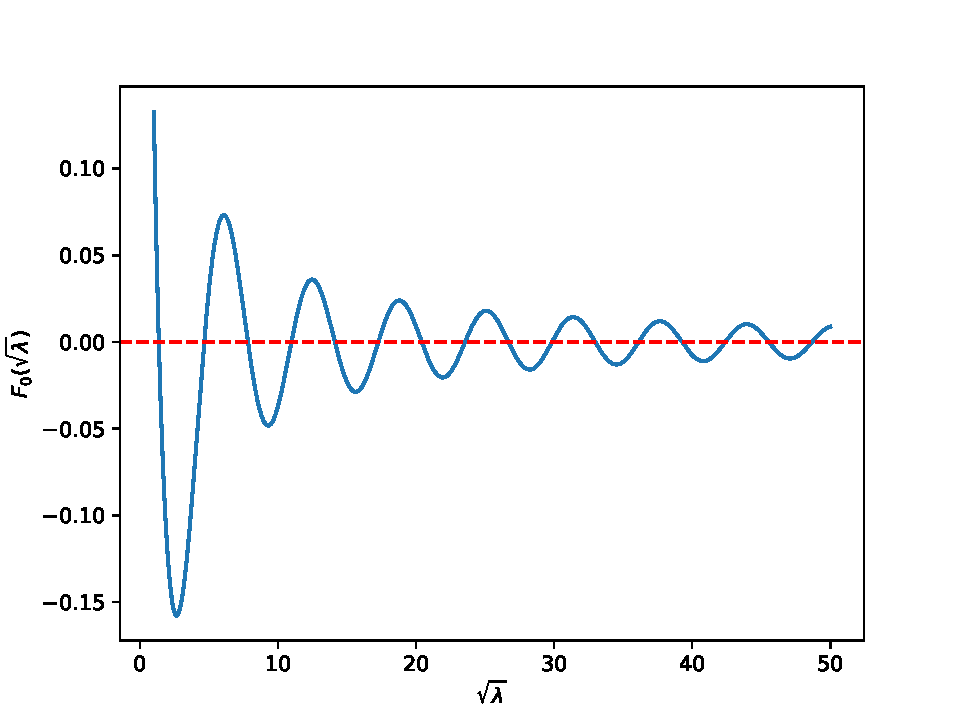
\includegraphics[width=0.5\textwidth]{F0}}%
  %\qquad
  \subfloat[]{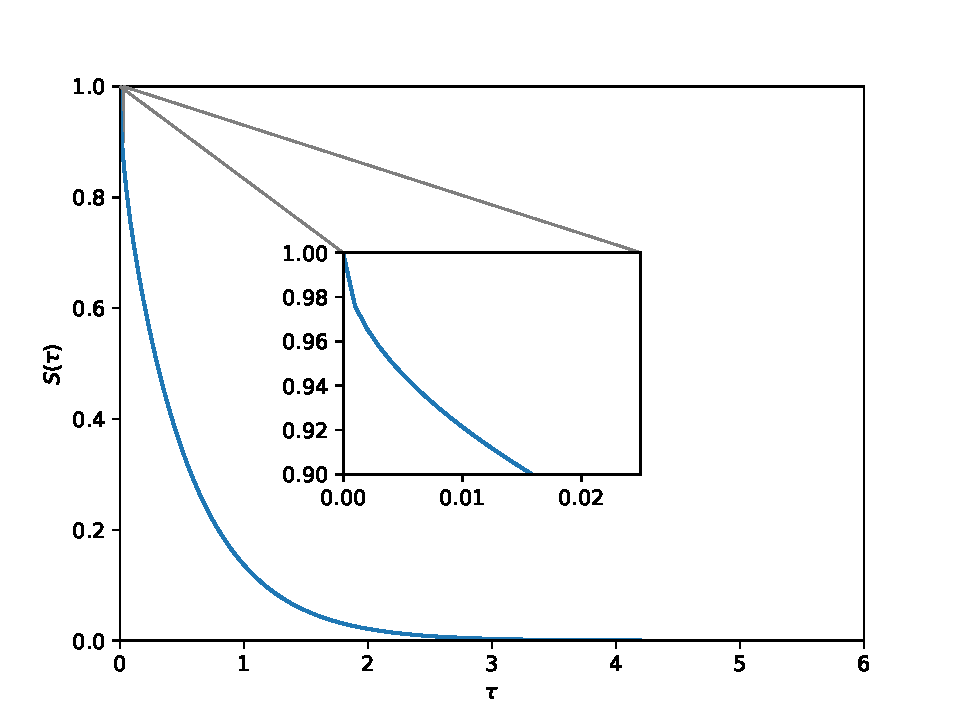
\includegraphics[width=0.5\textwidth]{analytical_s}}%
  \caption{(a) It is straightforward to evaluate the cross-product of
    Bessel fucntions by SciPy library \cite{2020SciPy-NMeth}. (b) The
    asymptotic behaviors of survival probability $S(\tau)$ are
    approximated by the numerical method with the first $1000$
    eigenvalues. $S(\tau)$ monotonously descrese from 1 at $\tau=0$ to
    $0$ as $\tau$ goes to infinity. Moreover, the approximation of
    analytical mean first-passage time $\langle \tau \rangle$ equals
    $0.47339248$.}
\end{figure}




 % subsection 2


  % ________ Section 3: Monte Carlo Simulations ________________________
  %\section{Monte Carlo Simulations}

In this section, several generally utilized numerical methods
\cite{grossmann2007numerical}\cite{zlamal1968finite}
\cite{eymard2000finite} \cite{attaway1991boundary} for solving the
heat equation, and their limitations in practice are presented. Also,
one of the non-deterministic algorithms, Monte Carlo methods (MCM)
\cite{rubinstein2016simulation} \cite{kroese2014monte}, and its
application in approximating the solution of the PDEs are proposed. As
the weaknesses and challenges of applying the numerical techniques in
solving $2-$dimensional heat equation defined in the real root images
with millions of pixels and extremely complex root systems, the
alternative fixed-time step Monte Carlo simulations, lattice random
walks (LRWs) and Pearson's random walks (PRWs), are designed. The most
outstanding advantage of the proposed random walk models is that the
integration, named the heat content, can be approximated directly
based upon the probabilistic interpretation of Brownian motion and the
heat equation.  Finally, the methods to analyze the output of the
Monte Carlo simulations and solve the sampling-related problems in the
simulations are brought up theoretically.



\subsection{Background}\label{background}

In the subsection~\ref{analytical results}, the analytical solutions
of the heat equation defined in the annulus with the initial and
boundary conditions have been derived. The analytical heat content,
calculated by the integration over $\Omega$, implies the geometrical
properties of the annulus. However, the analytical method for solving
the heat equation has many restrictions, and its applications to
practical problems will exhibit difficulties. Firstly, the numerical
evaluation of the analytical solutions is usually by no means trivial
because they are in the form of infinite series. Secondly, either
irregular geometries or discontinuities lead to the complexities, so
the explicit algebraic solutions are close to non-existed. Thirdly,
the purely analytical techniques can apply strictly only to the linear
form of the boundary conditions and to constant diffusion properties
\cite{crank1979mathematics}. Therefore, numerical methods and computer
simulations are more helpful and applicable to find solutions to the
heat equation than calculating pure analytical solutions.
 % subsection 1
      %\subsubsection{\highlight[id=Yuge, comment={The writing of this part has been revised. Dave, please give me the feedback or comments on it. }]{Numerical Methods}}\label{numerical methods}

The techniques for solving initial-boundary value problems (IBVPs)
based on numerical approximations have existed for a long time and
been developed considerably including the finite-difference method
(FDM), finite element method (FEM), finite volume method (FVM),
boundary element method (BEM), and so forth.


FDM is frequently utilized to converting the heat equation into a
system of algebraically solvable
equations \cite{grossmann2007numerical}. The basic idea is to replace
the derivatives in the equation by the difference quotients. For
example, the FTCS (Forward Time Centered Space)
scheme \cite{pletcher2012computational} discretize the Laplace
operator in space and the time derivative and implement the boundary
conditions on the staggered grid for representing the original
continuous problem, but it is conditionally
stable \cite{pletcher2012computational}. If the spatial resolution
becomes doubled, the time-step should be reduced by a factor of four
to maintain the numerical stability, which causes the extremely tiny
time-step in the high-resolution calculations. There are three kinds
of errors needed to be considered when using FDM. First of all, in the
derivation of the finite-difference equations, the higher-order terms
in the Taylor series are neglected, constituting the truncation
error. If the time and space interval tends to $0$, the truncation
errors will approach $0$, or the FDM is incompatible or inconsistent
with the original heat equation \cite{crank1979mathematics}. Another
class of error appearing in FDM, called round-off error, results from
the loss of precision due to the computer rounding of decimal
quantities. \cite{hoffman2018numerical}. The last type of error is the
discretization error, which can be reduced by decreasing the time
size, grid size, or both \cite{crank1979mathematics}. Moreover, DFM
becomes less accurate and hard to implement when the problem is
defined in the irregular geometries since the heat equation must be
transformed before applying the Taylor series.


Unlike the FDM, FEM \cite{zlamal1968finite} divides the complicated
and irregular geometries and boundaries into the union of smaller and
simpler subdomains or finite elements \cite{logan2011first},
e.g. lattice, triangle, curvilinear polygons, etc. Each subdomain is
locally represented by the element equation, continuous piecewise
shape functions, which are finally assembled into a larger system of
algebraic equations for modelling the entire problem. The numerical
solution can be obtained by minimizing the associated error function
to meet the certain specification of the accuracy. The smaller size of
the finite element mesh, the more accurate the approximate
solution. FEM has great flexibilities or
adaptivity \cite{reddy1993introduction}. For instance, FEM can provide
higher fidelity or accuracy in a specific local region and keep
elsewhere identical. Nevertheless, FEM requires an amount of human
involvement in building the FE model, checking the result, detecting
and updating the model design. Moreover, compared with FDM, FEM
demands a longer execution time and a larger amount of input data.


FVM, closely related to FEM, converts the original heat equation into
the integral forms \cite{eymard2000finite}. However, the accuracy of
FVM is related to the numerical integration over time and space
dimensions. Unlike the domain-type methods (e.g. FDM, FEM, FVM, etc.),
BEM transforms the heat equation into an integral equation over the
boundary of the domain using the boundary integral equation
method \cite{attaway1991boundary}. Especially, when the domain extends
to infinity or the boundary is complex, BEM is more efficient in
computation than other methods because of the smaller surface or
volume ratio \cite{katsikadelis2002boundary} since it only discretizes
the boundary and fits the boundary values into the integral
equation \cite{ang2007beginner}. However, it is arduous to solve the
matrics generated in BEM, since they are generally unsymmetric and
fully populated \cite{mushtaq2010advantages}.


In summary, all the described numerical methods have an intrinsically
similar feature - mesh discretization in the time and space
dimension. In this thesis, the heat equation is defined in a
$2$-dimensional domain, bounded by the border of the image and that of
the root system, with millions of pixels, the extremely complex roots
and various boundary conditions. It may be possible to calculate the
heat content contained in this domain by the numerical integration of
the solutions approximated by those numerical techniques. However,
some practical problems have to be taken into consideration. For
instance, the far more efforts are required when applying FDM and FVM
because of the complicated boundary of the roots and non-continuous
issues. Although the whole $2$-dimensional root image can be viewed as
a discretized domain, it is still time-consuming and challenging to
trace and identify the boundary of roots, label the nodes, and
generate the coordinates and connectivities among the nodes in the
preprocessing stage of FEM. The finer discretization, the more
accurate approximated solutions of the original IBVP and the longer
computational time spent by the numerical methods. More importantly,
the heat content, which is the integration of the numerical solution
over the space dimension, should also be approximated numerically
resulting in extra effort and errors.






      %\subsubsection{\highlight[id=Yuge, comment={This writing has been revised. Dave, please give me the feedback and comments. Thanks!}]{Probabilistic Interpretation}}\label{probabilistic interpretation}

In the subsection~\ref{analytical results}, the heat equation
describes the temperature distribution of a homogeneous and isotropic
domain \cite{varadhan1980lectures}, and its solution characterizes how
the temperature changes over the position and time. From the
probabilistic perspective, the heat equation and its solution can also
be understood by the Brownian
motion \cite{brown1828microscopical}. The Brownian motion also called
the Wiener process, is a continuous-time and continuous-space
stochastic process \cite{karlin2014first} with the continuous sample
paths and stationary independent
increments \cite{ito2012diffusion}. This process also has the Markov
property: the future state depends only on the present
state \cite{bharucha2012elements}. In the probability theory, if a
large number of free particles undergoing the Brownian motion
independently, the density of particles at a specific time becomes a
deterministic process called diffusion, which satisfies the heat
equation \cite{kac1947random}\cite{varadhan1980lectures}.



\paragraph{Survival Probability}


\newcommand{\prob}{P(\hat r, \theta, \tau | \hat{r_0}, \theta_0, 0)}
% Define the conditional probability u, which will be used frequently. 
                                 

For simplicity, we only investigate the probabilistic interpretation
of the heat equation defined in the annulus with the boundary and
initial conditions as same as described in the
subsection~\ref{analytical results}. Consider a particle undergoing
the Brownian motion from $(\hat{r_0}, \theta_0) \in \Omega$ at
$\tau=0$ and let $\prob$ be the conditional probability of finding the
particle at $(\hat r, \theta) \in \Omega$ at time $\tau>0$. $\prob$
satisfies the following equations

\begin{align}
  \frac{\partial \prob}{\partial \tau} &= \Delta \prob
  \qquad\text{for $(\hat r, \theta) \in \Omega$}\label{eq:polar_coordinate_diffusion_conditional_prob} \\
  \prob & = 0
  \qquad\text{for $(\hat r, \theta) \in \partial \Omega_1$}\label{eq:Dirichlet_bc_conditional_prob} \\
  \frac{\partial}{\partial \hat r} \prob &= 0 
  \qquad\text{for $(\hat r, \theta) \in \partial \Omega_2$}\label{eq:Neumann_bc_conditional_prob} \\
  \prob & = \frac{1}{\hat r}\delta(\hat r - \hat{r_0}) \delta(\theta - \theta_0)
  \qquad\text{for $\tau = 0$}\label{eq:initial_cd_conditional_prob}
\end{align}

Note, Eq.~\ref{eq:polar_coordinate_diffusion_conditional_prob} is the
heat equation and supplemented by the initial condition
Eq.~\ref{eq:initial_cd_conditional_prob} with the Dirac $\delta -$
distribution, absorbing boundary condition
Eq.~\ref{eq:Dirichlet_bc_conditional_prob}, and reflecting boundary
condition Eq.~\ref{eq:Neumann_bc_conditional_prob}. Similarly, the
conditional probability $\prob$ can be expressed in terms of the
eigenvalues and eigenfunctions. 

Define the local survival probability $S(\tau | \hat{r_0}, \theta_0,
0)$ as the probability that the particle, localized initially at
$(\hat{r_0}, \theta_0)$, keeps diffusing in $\Omega$ at time $\tau >
0$ without being absorbed by $\Omega_1$. It can be calculated by


\begin{equation}\label{eq:cpu_s_local}
  S(\tau | \hat{r_0}, \theta_0, 0) = \iint_{\Omega} \hat r \prob d \hat r d\theta
\end{equation}
  
Thus, the survival probability $S(\tau)$ for a particle, starting with
an initial distribution uniformly spread in $\Omega$, is the average
of the local survival probability over $\Omega$. It is

\begin{equation}\label{eq:cpu_s_global}
  S(\tau) = \frac{1}{|\Omega|}\iint_{\Omega} \hat{r_0} S(\tau | \hat{r_0}, \theta_0, 0) d \hat{r_0} d \theta_0
\end{equation}

Eq.~\ref{eq:cpu_s_local} and Eq.~\ref{eq:cpu_s_global} reveal that the
heat content $Q_{\Omega}(\tau)$ in Eq.~\ref{eq:annulus_analytical_s},
calculated as the integration of the temperature over $\Omega$, is
proportional to the survival probability
$S(\tau)$ \cite{kalinay2011survival}. 


\paragraph{Mean First-Passage Time}

The first passage phenomena play a fundamental role in the stochastic
processes triggered by a first-passage
event \cite{van1992stochastic}. In this thesis, the first-passage
event refers to the first time when the Brownian motion is stopped
because of the present of the Dirichlet boundary condition. One of the
essential first-passage-related quantities is the first-passage time
or the first-hitting time \cite{redner2001guide}, which is the time
taken by particle undergoing the Brownian motion from an initial
position to any sites of $\Omega_1$ for the first time. Particles'
mean first-passage time $\langle \tau \rangle$, also called the
average first-passage time, has a closed relationship with the
survival probability $S(\tau)$ \cite{redner2001guide}

\begin{equation}\label{eq:mfpt_conditional_prob}
  \begin{split}
    \langle \tau \rangle &= \int_{0}^{\infty} \tau dS(\tau)\\
    &=\sum_{n=1}^{\infty} \frac{4}{\mu^2 - 1}
    \frac{1}{\lambda^2_{0,n}\bigg\{\bigg[\frac{J_0(\sqrt{\lambda_{0,n}})}{J'_0(\mu\sqrt{\lambda_{0,n}})}\bigg]^2
      -1\bigg\}}
  \end{split}
\end{equation}


From Eq.~\ref{eq:mfpt_conditional_prob} and
Eq.~\ref{eq:eigenfunction}, it is clear that $\langle \tau \rangle$
implies an overall property of the annulus since it only depends on
the radius ratio of annulus $\mu$.


\paragraph{Brownian Motion and Random Walks}

Brownian motion, the irregular motion of individual particles, has
been existed for a long time before the random-walk theory was
developed. At the beginning of the twentieth century, the term, random
walk, was initially proposed by Karl
Pearson \cite{pearson1905problem}. He utilized the isotropic planar
random flights to model how mosquitoes migrate and invade randomly in
the cleared jungle regions. At each time step, the mosquito moves to a
random direction with a fixed step
length. Rayleigh \cite{rayleigh1905problem} answered Pearson's
question in the same year, that is, the distributions of mosquitos
after many steps have been taken is identical to superposition the
sound vibrations with unit amplitude and arbitrary
phase \cite{de2012flying}. At almost the same time, Louis
Bachelier \cite{bachelier1900theorie} designed a model for the
financial time series based on the random walks. Louis Bachelier also
explored the relationship between discrete random walks and the
continuous heat equation. During the development of random-walk
theory, many other scientific fields, including the random processes,
random noise, spectral analysis, and stochastic equations, were
developed by some
physicists \cite{einstein1905electrodynamics} \cite{einstein1906theory} \cite{smoluchowski1916drei}. The
continuous Brownian motion is the scaling limit of the discrete random
walks as the time and space increments approach
zero \cite{lawler2010random}\cite{varadhan1980lectures}.


\paragraph{Lattice Random Walks (LRWs)}

\newcommand{\p}{p(x,y,t)}


Let us consider a particle performing the simple random walk on the
$d$-dimensional integer grid $\mathbb{Z}^d$. It is a discrete-space
and discrete-time symmetric hopping process \cite{redner2001guide} on
the lattice. At each time step, the particle moves to one of its $2d$
nearest neighbours with probability $\frac{1}{2d}$. If $d \leq 2$, the
random walk is recurrent, which means the
particle will return to its origin infinitely often with the
probability $1$. If $d \geq 3$, the random walk is
transient, which indicates the particle will
return to its origin only finitely often with the probability
$1$ \cite{hughes1998random} \cite{lawler2010random}. Only $2$-dimensional lattice random walks
(LRWs) and its connection with the heat equation are introduced since
this thesis aims to explore and characterize the shape of roots in the
$2-$dimensional images.

Let $\triangle l$ be the distance between two sites in the lattice and
$\delta$ be the time step. Let $p(i, j, n)$ be the probability of
finding a particle to be in position $(i, j)$ after $n$ steps. There has

\begin{equation}\label{eq:p_ijn}
p(i, j, n) = \frac{p(i-\triangle l, j, n-1) + p(i + \triangle l, j, n-1) + p(i, j - \triangle l, n-1) + p(i, j + \triangle l, n-1)}{4}
\end{equation}

\begin{align}\label{eq:p_diff}
p(i, j, n) - p(i, j, n-1) & = \frac{1}{4}\left(p(i-\triangle l, j, n-1) - 2p(i,j, n-1) + p(i + \triangle l, j, n-1)\right) \notag \\
&\quad + \frac{1}{4}\left(p(i, j - \triangle l, n-1) - 2p(i,j, n-1) + p(i, j + \triangle l, n-1)\right)
\end{align}


\begin{align}
x &= i \triangle l \label{eq:x}\\
y &= j \triangle l \label{eq:y}\\
t &= n \delta \label{eq:t}
\end{align}

Eq.~\ref{eq:x} and Eq.~\ref{eq:y} can be used to definde particle's position in the $x-y$ coordinate system and Eq.~\ref{eq:t} is the walking time taken by the particle after $n$ steps.

\begin{align}
p(i, j, n) - p(i, j, n-1) &= p(x, y, \frac{t}{\delta}) - p(x, y, \frac{t-\delta}{\delta}) \\
& \approx \delta \frac{\partial \p}{\partial t} \label{eq:t_diff}
\end{align}

Similarly,

\begin{align}
p(i-\triangle l, j, n-1) - 2p(i,j, n-1) + p(i + \triangle l, j, n-1) & \approx (\triangle l)^2 \frac{\partial^2 \p}{\partial x^2}\label{eq:x_diff}\\
p(i, j - \triangle l, n-1) - 2p(i,j, n-1) + p(i, j + \triangle l, n-1) & \approx (\triangle l)^2 \frac{\partial^2 \p}{\partial y^2}\label{eq:y_diff}
\end{align}

Aftering substitue Eq.\ref{eq:t_diff}, Eq.~\ref{eq:x_diff}, and Eq.~\ref{eq:y_diff} into Eq.~\ref{eq:p_diff}, $p(x,y,t)$, the probability of particle at $(x, y)$ at time $t$, satisfies

\begin{equation}\label{eq:lrws_heat}
  \frac{\partial \p}{\partial t} = \frac{(\triangle
    l)^2}{4 \delta} (\frac{\partial ^2 \p}{\partial x^2} +
  \frac{\partial^2 \p}{\partial y^2})
\end{equation}

where $D = \frac{(\triangle l)^2}{4 \delta}$ is the diffusion
coefficent. This above derivation shows a tight relationship between
the $2-$ dimensional discrete lattice random walks and the heat
equation.


\paragraph{Pearson's Random Walks (PRWs)}

Based on Pearson's problem and Rayleigh's answer,
Stadje \cite{stadje1987exact} and Masoliver et
al. \cite{masoliver1993some} considered a two-dimensional
continuous-time and continuous-space random walk, defined as Pearson's
random walks (PRWs) in this thesis. In PRWs, particle moves with
constant speed and with random directions distributed uniformly in
$[0, 2\pi)$. Moreover, the lengths of the straight-line paths and the
turn angles are stochastically independent. If the mean step length
approaches zero and the walking time is big enough, the behaviours of
particles in PRWs weakly converges to the Wiener
Process \cite{stadje1987exact}, which satisfies the traditional heat
equation. 

      %\subsubsection{Monte Carlo Simulations For Solving PDEs}

Monte Carlo methods (MCMs), the commonly used computational techniques, aim to generate samples from a given probability distribution, estimate the functions' expectations under this distribution, and optimize the complicated objective functions by using random numbers \cite{kroese2014monte} \cite{rubinstein2016simulation}. MCMs can be used to solve the IBVPs by generating the random numbers to simulate the successive positions of the trajectory of a stochastic process at fixed instants \cite{kronberg1976solution}\cite{king1951monte}, since the original continuous problem can be represented by the probabilistic interpretation and the solution can be approximated by the expectation of some functional of the trajectories of a stochastic process \cite{grebenkov2014efficient}\cite{sabelfeld2013random}. Therefore, unlike the numerical techniques proposed in the subsubsection~\ref{numerical methods}, the nondeterministic Monte Carlo simulations are grid-free on the domain, boundary, and the boundary conditions of the problem \cite{grebenkov2014efficient}.


Monte Carlo simulations have been applied frequently in solving the elliptic partial differential equation, for example, the Laplace’s and Poisson’s equations \cite{haji1967application} \cite{booth1981exact} \cite{muller1956some}. For example, let $u(P_0)$ be the value of the solution of the elliptic partial differential equation at a specific point $P_0$ in a bounded domain. $u(P_0)$ can be estimated by a point $P_1$, which is sampled uniformly on the largest circle $C_0$ centered at $P_0$ with radius $r_0$ lying entirely in the domain. If $P_1$ gets closed to the target bounday within an error, $u(P_1)$ is known, and it can be considered as a particle's estimate of $u(P_0)$ by multiplying the particle’s statistical weight. If not, $u(P_1)$ is should be estimated in the same way as $u(P_0)$, that is, $P_2$ is sampled uniformly on the largest circle $C_1$ centered at $P_1$ with radius $r_1$ lying entirely in the domain. Check the position of $P_2$, and the procedure will be repeated until the simulation is terminates on the traget boundary, which is defined as one particle's estimate of $u(P_0)$. Finally, averaging a larger number of one-particle estimates, $u(P_0)$ will be more accurate. 


However, Monte Carlo simulations are barely applied in solving parabolic and hyperbolic partial differential equations, such as the $1-$ dimensional and $2-$ dimensional time-dependent heat problem. As introduced in the papers \cite{sadiku2006monte} \cite{gemjoz2017mcmheat}, after obtaining the probabilistic interpretation of the finit-difference approximation of the heat equation, the solution of the heat equation at a specific space-time point can be approximated by averaging a large number of random-walking particles, whose trajectories are simulated by the Monte Carlo methods untill they hit the any sites of the target boundary. However, the drawbacks of this method are obvious. Firstly, there is the error appeared in the finit-difference approximation. Secondly, there has the statistical sampling errors inherent in the Monte Carlo simulations. Last but not least, it will be time-comsuming to evaluate the solution defined in the whole domain, the real root images with millions pixels in this thesis, since this method can only be used to approximate the solution of the heat equation at one point at a time. 











  %\subsection{Algorithms of Random Walks}

In the subsection~\ref{background}, the practical challenges of
solving the heat equation defined in the $2-$ dimensional domain with
the complicated root systems by numerical methods and Monte Carlo
simulations are revealed, and the probabilistic interpretation of the
heat equation, survival probability, and random walks are introduced.
From Eq.~\ref{eq:annulus_analytical_s}, Eq.~\ref{eq:cpu_s_global}, and
Eq.~\ref{eq:mfpt}, the final goal in this thesis is to approximate the
heat content, or the survival probability, defined as the integrals,
which only depends on the time variable. In other words, our interest
is only related to the time when the first-passage event happens in
the stochastic process, that is, the first-passage time. Therefore, in
this subsection, two random walks algorithms are designed to mimic
particles' first-passage time by $2-$ dimensional fixed-time step
Monte Carlo simulations in the real root images for approximating the
integration as expressed in Eq.~\ref{eq:cpu_s_global} and
Eq.~\ref{eq:mfpt}.


\subsubsection{Lattice Random Walks}


  \begin{algorithmic}
    \caption{Lattice Random Walks (LRWs)}\label{lrws_algorithm}
    \floatname{algorithm}{Procedure}
    \renewcommand{\algorithmicrequire}{\textbf{Input:}}
    \renewcommand{\algorithmicensure}{\textbf{Output:}}

  \end{algorithmic}






\subsubsection{Pearson's Random Walks}

\begin{algorithm}
  \caption{Pearson's Random Walks (PRWs)}\label{prws_algorithm}
  
\end{algorithm}
 % subsection 2
      
  %\subsection{Output Analysis}

The output of the fixed-time step Monte Carlo simulations are particles' first passage time $t$, which is the number of steps taken by the particles hitting any positions of the target for the first time. Since first-hitting-time models are a sub-class of survival analysis in statistics \cite{altman1990practical}, it is straightforwad to use the Kaplan-Meier estimator to estimate the survival function $S(t)$ \cite{kleinbaum2005competing} of the numerical simulation, which provide the probability that a particle remains wandering beyound any specified time. Moreover, the pointwise upper and lower confidence interval can also calculatated by the Greenwood’s exponential formula \cite{hosmer2011applied}. In this subsection, the Kaplan-Meier estimator and confidence interval of $S(t)$ are introduced theoretically. However, in practice, the existed Python module, lifeline \cite{davidson2019lifelines}, will be used to implement the estimation. After obtaining the estimated survival function of the fixed-time step Monte Carlo simulations, the scaling relationship between $t$ and $\tau$ is derived for the valiation of research methodology in the next chapter.
 % subsection 3
      %\subsubsection{Kaplan-Meier Estimator}

The general definition of the survival time is the time starting from a specified point to the occurrence of a given event \cite{bewick2004statistics}, such as death, pregnancy, job loss, etc. Also, the analysis of the group of survival data is called survival analysis \cite{altman1990practical}. In the survival analysis, three kinds of situations will affect the subjects' survival time \cite{goel2010understanding}. Firstly, the subjects are uncooperative and refused to continue to participate in the research. Secondly, some subjects do not experience the event before the end of the study, but they would have experienced the event if they keep being observed. Finally, the researchers lose touch with the subjects in the middle of the investigation. In practice, since these subjects have partial information about survival, the scientists will label the above circumstances as censored observations \cite{bewick2004statistics} instead of ignoring them and decreasing sample size.

In clinical trials or community trials, Kaplan-Meier Estimator \cite{kaplan1958nonparametric}, a non-parametric analysis, is a commonly applied statistical method in the survival analysis for the measurement of the fraction of the survival time after the treatment \cite{aalen2008survival} and for generating the corresponding survival curve. It also works well with the mentioned three difficult
situations. With various assumptions \cite{etikan2017kaplan} \cite{goel2010understanding}, the Kaplan-Meier survival curve can be created and provides the probability of surviving in a given length of time while considering the time in many small intervals \cite{altman1990practical}.


Let $0 < t_1 < t_2 < ...$ be the distinct increasing observed times, or the number of steps taken by the particle countering the absorbing boundary, in the sample. Let $n_i$ be the number of particles who either have not yet stopped moving up to time $t_i$ or else who are absorbed on the target boundary at time $t_i$ in the simulations. Let $d_i$ the number of particles hitting the target boundary at time $t_i$. The Kaplan-Meier or product-limit estimator $\widehat{S}(t)$ of the survival function of the numerical simulation $S(t)$ is \cite{aalen2008survival}

\begin{equation}
  \widehat{S}(t) = \prod_{i:t_i \leq t} (1 - \frac{d_i}{n_i})
\end{equation}





      %\subsubsection{Confidence Interval}

The upper and lower $(1-\alpha) \times 100 \%$ confidence intervals of the survival function $S(t)$ for a fixed time $t$ was firstly proposed and derived by Greenwood in 1926 \cite{greenwoodnatural},


\begin{align} \label{eq:greenwood}
  \widehat{S}(t) \pm z_{\alpha / 2} \sqrt{\widehat{Var}[\widehat{S}(t)]}
  \qquad\text{where}\\
  \widehat{Var}[\widehat{S}(t)] = \widehat{S}(t)^2\sum_{t_i \leq t} \frac{d_i}{n_i(n_i - d_i)}
\end{align}

Note, $z_{\alpha}$ is the $\alpha -$th quantile of the normal distribution.

In 1999, Hosmer and Lemeshow \cite{hosmer2011applied} developed the exponential Greenwood formula based on the earlier works of Kalbfleisch and Prentice \cite{kalbfleisch2011statistical}, which provides an asymmetric confidence interval for $S(t)$

\begin{align} \label{eq:exp_greenwood}
  e^{-e^{c_{+}(t)}} < S(t) < e^{-e^{c_{-}(t)}}
  \qquad\text{where}\\
  c_{\pm}(t) = log(-log\widehat{S}(t)) \pm z_{\alpha / 2} \sqrt{\widehat{V}}
  \qquad\text{and}\\
  \widehat{V} = \frac{1}{(log\widehat{S}(t))^2} \sum_{t_i \leq t} \frac{d_i}{n_i(n_i - d_i)}
\end{align}

Note, if $c1<c2$, there has $e^{-e^{c_2}} < S(t) < e^{-e^{c_1}}$.


Compared with the traditional Greenwood confidence intercal calculation, the exponential Greenwood formula will make sure that the endpoints in Eq.~\ref{eq:exp_greenwood} lie in $(0, 1)$, while the endpoints in Eq.~\ref{eq:greenwood} could be negative or larger than $1$ \cite{sawyer2003greenwood}. 





      %\subsubsection{Relationship between $t$ and $\tau$}

Particles' average one-step displacement $\triangle l$ in the
fixed-time step Monte Carlo simulations, LRWs and PRWs, are associated
with the time step is $\delta$:

\begin{equation}\label{eq:scaling_relationship}
  \triangle l = 2 \sqrt{D \delta}
\end{equation}
where $D$ is the diffusion coefficent.

Eq.~\ref{eq:scaling_relationship} implies that the time step $\delta$
must be designed small enough to make sure that $\triangle l$ is
shorter than the smallest geometrical features of the
boundaries. Thus, $\triangle l$ should equal or be less than one-pixel
size in the simulations. Furthermore, the $\delta$ is regarded as a
fundamental bridge between particles' number of steps $t$ and unitless
continuous-time $\tau$,

\begin{equation}\label{eq:tau}
 \tau = t \delta = \frac{(\triangle l)^2 t}{4D}
\end{equation}
where $D$ is 1.

When running the LRWs in the annulus, $\triangle l$ is always
$\frac{1}{100}$ since particle's step length is as same as one-pixel
size. However, $\triangle l$ is related to the particle's step length
in PRWs. If particle's step length is $0.5$, a half of a pixel, then
$\triangle l$ equals $\frac{1}{100} \times \frac{1}{2} =
\frac{1}{200}$.  Similiarly, when the step length in PRWs is $0.1$,
then $\triangle l$ is $\frac{1}{1000}$. 


  %\subsection{Sample Size Determination}

Based on the law of large number (LLN) \cite{dekking2005modern}, as
the sample size approaches infinity, the sample mean tends to get
closer to the true population mean with the high
probability. Moreover, the central limit theorem (CLT)
\cite{dekking2005modern} illustrates how the sampling distribution of
the mean changes as a function of the sample size and how much more
reliable a large experiment is. On the downside, the increasing number
of trials results in the higher cost of performing the simulation,
which is the major drawback of the fixed time-step Monte Carlo
simulations. Therefore, it is necessary to conduct the minimum number
of simulation runs to achieve a desired degree of precision.
 % subsection 4
      %\subsubsection{General Method}

There are five parts of the standard way to determine the sample size
in the Monte Carlo simulations. Firstly, simulating with a certain
amount of samples. Secondly, repeating the simulation several times
with the sample size as the same as the first step.  Thirdly,
increasing the number of samples and implementing the first two steps
again. Fourthly, running a regression analysis of the variability of
the sample statistic as a function of sample size. Finally, estimating
the sample size that will result in any desired level of convergence
by some probabilistic inequalities, including Chebyshev's inequality
\cite{chebyshev1867valeurs}, Cantelli’s inequality
\cite{cantelli1929sui}, Vysochanskij–Petunin inequality
\cite{vysochanskij1980justification}, etc.

      %\subsubsection{Dvoretzky–Kiefer–Wolfowitz (DKW) inequality}

Although the sample size estimated by the general method does not
depend on the geometries characterized by the random walk models, how
long the simulation will run is unknown, and the final calculated
sample size will be larger than the really necessary value
sometimes. Therefore, an alternative method, named the
Dvoretzky–Kiefer–Wolfowitz (DKW) inequality
\cite{dvoretzky1956asymptotic}, is proposed for the sample size
determination without simulating random walk models and considering
the shape of objects in the images.

Let $F_N(x)$ denote the empirical distribution functions (empirical
CDF) for a sample of $N$ real-valued $i.i.d.$ random variables,
$X_{1}, ... , X_{N}$, with continuous cumulative distrbution function
(CDF) $F(x)$. The DKW inequality, as expressed in Eq.$(2.18)$, bounds the
probability that the random function $F_{N}(x)$ differs from the true
$F(x)$ by more than a given constant $\varepsilon$
\cite{dvoretzky1956asymptotic}.

\begin{equation}
  Pr(\sup_{x \in \mathbb{R}} |F_{N}(x) - F(x)| > \varepsilon) \leq
  2e^{-2N\varepsilon^2} \;\; \;\; for \; every \; \varepsilon > 0
\end{equation}

The equally spaced confidence bounds or simultaneous band around the
$F_{N}$ encompassing the entire $F(x)$ can be expressed by
\begin{equation}
  F_{N}(x) - \varepsilon \leq F(x) \leq F_N(x) + \varepsilon \; \; \; \; 
\end{equation}

On the other hand, assume the simultaneous band produced by Eq.$(2.19)$
containing the $F(x)$ at a given confidence level $1-\alpha$, the
interval $\varepsilon$ can be calculated by

\begin{equation}
  \varepsilon = \sqrt{\frac{\ln{\frac{2}{\alpha}}}{2N}}
\end{equation}


Given a converge probability $\alpha$ and constant $\varepsilon$, it is
straightforward to estimate the sample size $N$ in the fixed-time step
Monte Carlo simulations in any images by Eq.$(2.20)$.


    
  % ________ Section 4: Two-Sample Statistical Tests ___________________
  %\section{Two-sample Statistical Tests}\label{statistical tests}

The differences between the survival curves generated by the
Kaplan-Meier estimator are visible sometimes. However, the
dissimilarities won't be easily detected by eyes if the survival
curves are overlapping over some parts or crossing at some time
points.  Since the Kaplan-Meier estimator does not provide any
information on whether two groups of survival data are statistically
similar or different, some popular statistical tests used specially in
the survival analysis course are presented in this section. Which test
should be selected in a specific circumstance is always debated
because there is a fine line between the statistical tests in the
survival analysis. Therefore, acknowledging the data in hand and
identifying the assumptions well is a prerequisite to determine the
tests appropriately.

Before listing the pros and cons of several statistical tests, the
censored survival times will be recalled firstly, which indicates the
time at which a subject is unobserved and the time to the event of a
subject is not recorded \cite{etikan2018choosing}. In this thesis, it
is possible to appear the censoring observation in the beginning or at
any other moment during the Monte Carlo simulations. If the simulation
finished, but the particle did not reach the target boundary, the
particle will be regarded as a right-censored. When the particle is
abandoned and not been observed during the simulations, it is termed
the random right censoring \cite{etikan2018choosing}. Another cause of
a deficient observation of particles' survival times is the left
censoring, which hints that the particles had stopped diffusing before
the simulation began. For instance, the particle is generated in or on
the pixels of roots. As mentioned in the last section, the
Kaplan-Meier method can still cope well with the right-censored and
left-censored observations in output.


In survival analysis, as the time interval gets close to $0$, the
instantaneous hazard rate can be calculated by limiting the number of
events per unit time divided by the number of events at risk
\cite{case2002interpreting}. The hazard ratio is an estimate of the
hazard rate in one group relative to that in another group
\cite{singh2011survival}. If the survival curves are parallel with the
identical shape, the hazard ratio is constant at any interval of
time. In this situation, the log-rank tests, also named the
Mantel-Haenszel, are reliable \cite{custodio2007diagnostics}.

If the hazard ratio does not satisfy the assumption, the log-rank test
will not be powerful to detect the differences in the survival
functions. In such a case, the Gehan-Breslow-Wilcoxon test, also
called Gehan’s generalized Wilcohon procedure, should be considered
alternatively \cite{agarwal2012statistics}. Also, under the constant
hazard ratio assumption, the Wilcoxon tests might be more reliable
than the log-rank tests \cite{custodio2007diagnostics}. The former one
gives more weight to the early failures, but the latter one is more
suitable for comparing the later events in the data
\cite{custodio2007diagnostics}. Generally, some general non-parametric
tests, based on the rank ordering (e.g. Mann-Whitney U test,
Kruskal-Wallis, etc.), are not always feasible in censoring survival
data \cite{agarwal2012statistics}. However, Gehan’s generalized
Wilcohon test is still robust when the censoring rates are low, and
the censoring distributions of groups are equal
\cite{karadeniz2017examining}.


Neither log-rank test nor Gehan’s generalized Wilcohon test can work
well when the survival curves cross while the Tarone-Ware test should
be chosen \cite{leton2001equivalence}. It pays more attention to the
failures happening somewhere in the middle of study
\cite{etikan2017kaplan}. Moreover, there is no limitation of the
number of groups when the Tarone-Ware test is applied
\cite{custodio2007diagnostics}. Similarly, the Fleming-Harrington test
is also accessible and robust for testing the differences between two
or more survival curves in the right-censored data based on the
counting process \cite{harrington1982class}.
















  % ________ Section 5: Research Design ___________________
  %\section{Research Design}
...
\subsection{Methodology}

\subsection{Idea}





%%%%%%%%%%%%%%%%%%%%%%%%%% CHAPTER 3 %%%%%%%%%%%%%%%%%%%%%%%%%%%%%%%%%%
  
%\chapter{Fixed-time Step Monte Carlo Simulations on Artificial Images}

  %__________ Section 1: Background _______________________
  %\section{Background}

...

\subsection{Purposes}

\subsection{Shape Design}

\subsection{Branching Structures}

  
  %__________ Section 2: methodology_validation _______________________

  %\section{Methodology Validation}

In the last chapter, the survival probability $S(\tau)$ and the mean
first-passage time has been calculated by solving the heat equation
and approximated by the numerical methods. Lattice Random Walks (LRWs)
and Pearson's Random Walks (PRWs) are implemented in the annulus
image, as shown in Figure~\ref{fig:annulus}, in Python. This section
aims to validate the research methodology by comparing the estimated
survival functions $S(t)$ of the numerical data with the analytical
solutions $S(\tau)$ where $t$ is the number of steps taken by the
particles in the fixed-time step Monte Carlo simulations and $\tau$
denotes the unitless time.


\subsection{Statistical Fluctuation Analysis}

Fixed-time step Monte Carlo simulations, LRWs and PRWs, are the
nondeterministic numerical representations of the original statistical
problem defined in the continuous-time and continuous-space with
numerous inputs and discrete-time trajectories. In the simulations,
the initial positions of the enormous number of particles and their
moving directions at each time step are determined by the randomly
uniform sampling. Thus, it is inevitable to appear the statistical
fluctuations, also called variance, defined as a measure of the
discrepancies between the estimate and the true solution. The
brute-force way to reduce the statistical fluctuations is to increase
the sample size.


The first kind of error stems from the sampling. As shown in
Figure~\ref{fig:annulus_32_particles} and
Figure~\ref{fig:annulus_256_particles}, the larger sample size in the
simulations, the estimated survival functions will be more
precise. LRWs are used to mimic the continuous-time and
continuous-space diffusion process by generating the discrete random
trajectories in the discrete time, which results in the
time-discretization and space-discretization errors. Although PRWs is
a model defined in continuous-time and continuous-space, the random
paths demand much longer time simulation as shown in
Figure~\ref{fig:annulus_finer_steps}.

\begin{figure}
  \begin{subfigure}{0.9\textwidth}
    \centering
    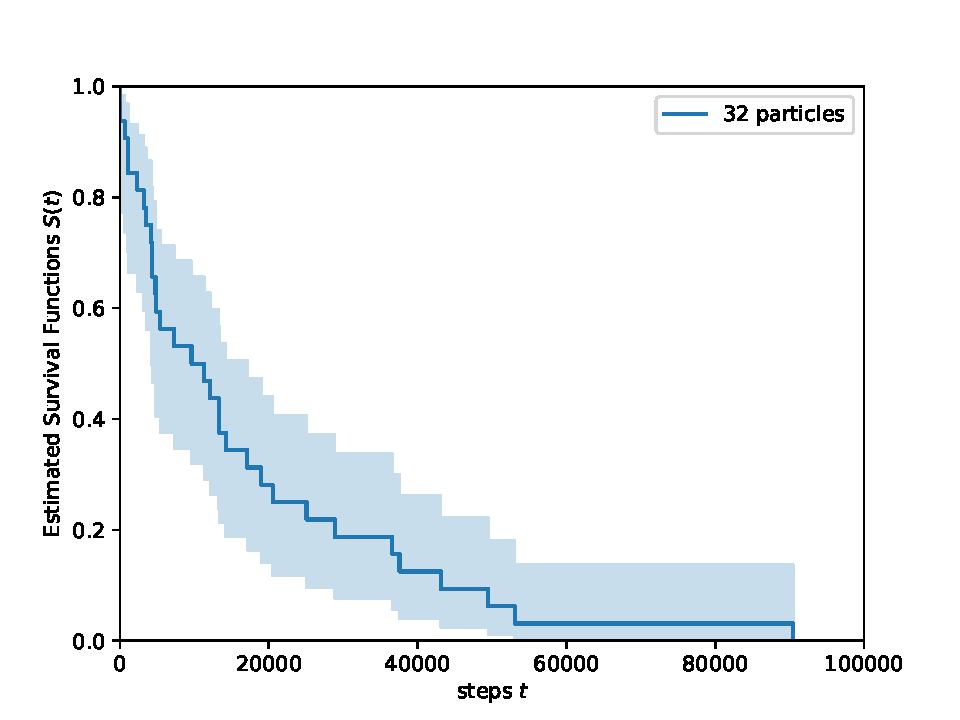
\includegraphics[width=0.8\textwidth]{sampling_32}
    \caption{Survival curve for the LRWs with $32$ particles.\label{fig:annulus_32_particles}}
  \end{subfigure}
  \begin{subfigure}{0.9\textwidth}
    \centering
    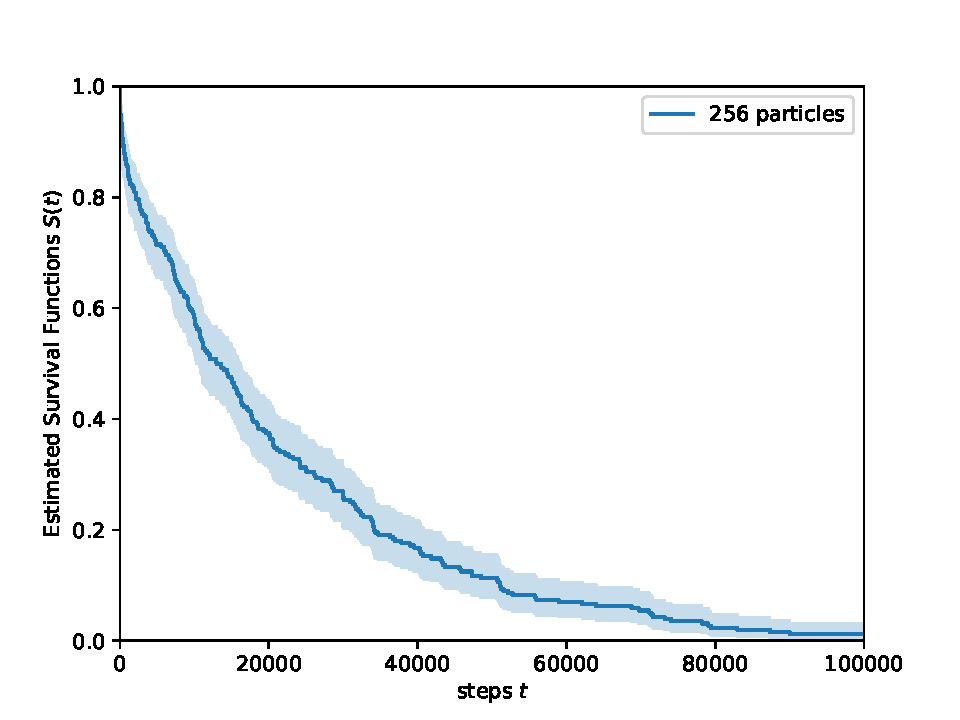
\includegraphics[width=0.8\textwidth]{sampling_256}
    \caption{Survival curve for the LRWs with $256$ particles. \label{fig:annulus_256_particles}}
  \end{subfigure}
  \caption{Estimated survival curves and 95\% confidence intervals for
    Monte Carlo simulations of partical diffusion on an annulus. As
    the number of particles increasing, the uncertainty of the LRWs
    simulation are lower since the confidence band of the estimated
    survival function becomes narrower.\label{fig:lrw_prw_annulus}}
\end{figure}



\begin{figure}
  \centering
  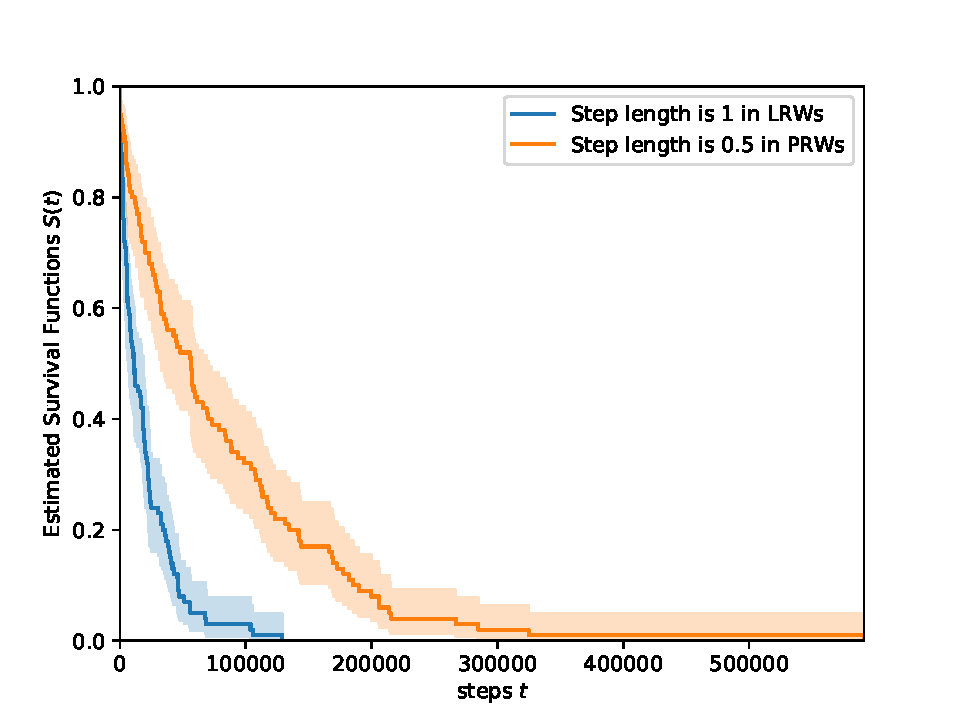
\includegraphics[width=0.8\textwidth]{discretization}
  \caption{When run LRWs and PRWs in the annulus with $100$ particles,
    the finer discretization step results in the longer simulation
    time.\label{fig:annulus_finer_steps}}
\end{figure}
 % subsection 1
  %

\subsection{Sample Size Determination and Evaluation}

In the last chapter, two approaches used to determine the appropriate
sample size in the fixed-time step Monte Carlo simulations have been
proposed. One of them is based on inferential statistics
\cite{casella2002statistical}, which infers and estimates the unknown
population parameters from the sample statistics. Another one is
simpler since it does not need any simulations.

\subsubsection{Chebyshev's inequality}

According to LLN \cite{dekking2005modern}, the unknown population mean
first-passage time $\bar X$ can be estimated by sample mean $\bar X_N$
when $N$ is big enough. Chebyshev’s inequality
\cite{chebyshev1867valeurs} is a probabilistic inequality that can be
applied to any probability distribution of a random variable with the
finite expected value and non-zero variance. This inequality provides
an upper bound to the probability that the absolute deviation of a
random variable from its mean will exceed a given threshold.

\begin{figure}
  \begin{subfigure}{0.9\textwidth}
    \centering
    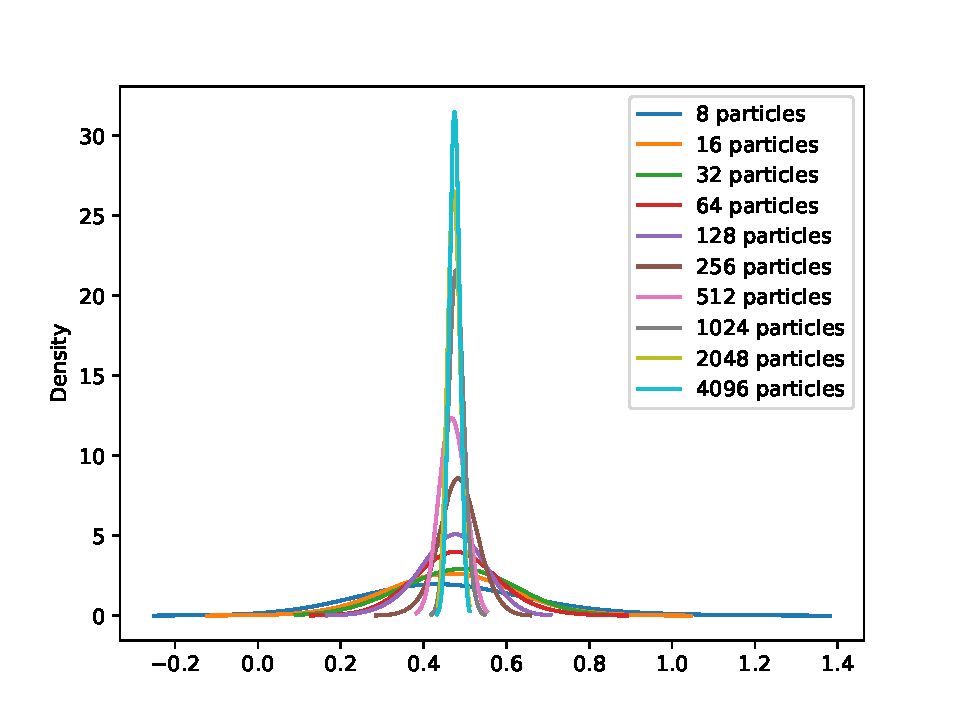
\includegraphics[width=0.9\textwidth]{kde}
    \caption{Running the LRWs in the annulus with $N = 2^i$
      particles and calculating the mean first-passage time $X_N$, where
      $i=3, 4, 5, ..., 12$. For each $N$, replicating the simulation
      $50$ times and recalculating the mean of the mean first-passage
      time $\bar X_{N}$ and the variance $\sigma^2_{N}$. As the sample
      size $N$ increase, the distribution of the sample means $X_N$
      becomes narrower and approximately normal. \label{fig:annulus_kde}}
  \end{subfigure}
  \begin{subfigure}{0.9\textwidth}
    \centering
    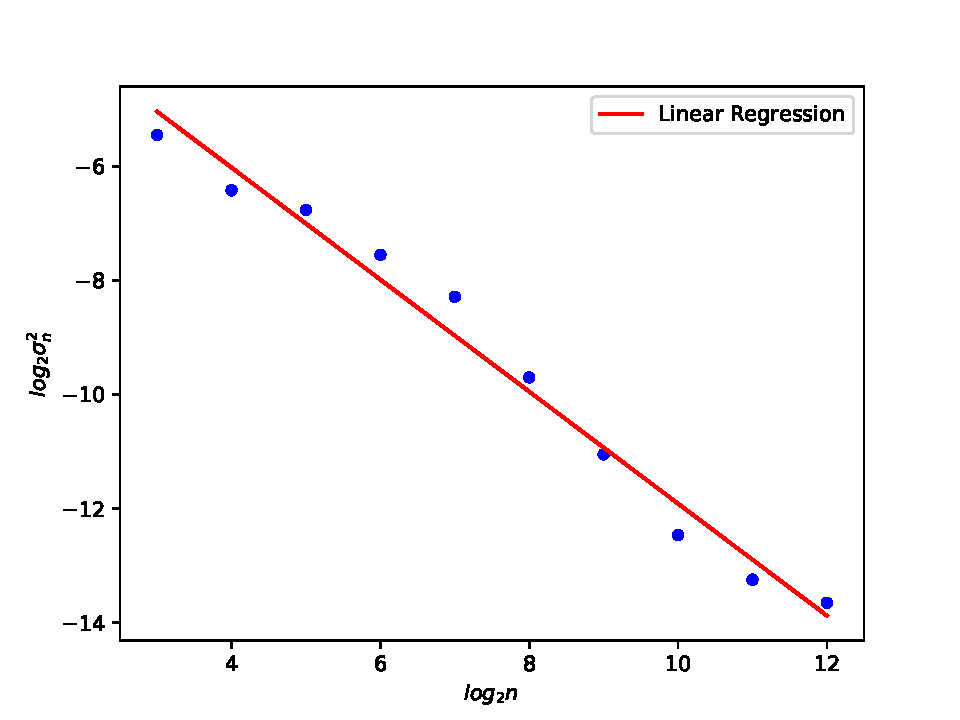
\includegraphics[width=0.8\textwidth]{linear_regression}
    \caption{A fitted linear regression model is used to explore the
      scaling relationship between $log_{2} (\sigma^2_{N})$ and
      $log_{2} N$. $log_{2} (\sigma^2_{N}) \approx b + k log_{2} N$,
      where $k$ and $b$ are the estimated model parameters, slope and
      intercept, respectively.\label{fig:annulus_linear_regression}}
  \end{subfigure}
  \caption{\label{fig:annulus_cheb}}
\end{figure}


In the Figure~\ref{fig:annulus_cheb}, the number of steps $t$ in the
numerical simulations have been converted into the unitless time
$\tau$ by the \highlight[id=Yuge, comment={No hard
    number}]{Eq.$(2.16)$}. Thus, given a predesignated error
$\epsilon$, the required number of particles $N$ can be determined by

\begin{equation}\label{eq:chab_substitute}
  Pr(|X_{N} - \bar X| \geq \epsilon) = Pr(|X_{N} - \bar X_{N}| \geq
  \epsilon) \leq \frac{\sigma^2_{N}}{\epsilon^2} \approx \frac{2^b
    N^k}{\epsilon^2} = 0.01
\end{equation}

where $\epsilon = 0.01 \bar X$.

The required number of particles in LRWs and PRWs can be estimated by
Eq.~\ref{eq:chab_substitute}, which is

\begin{equation}\label{eq:cheb_sample_size}
  N \geq (\frac{0.01 \epsilon^2}{2^b})^{\frac{1}{k}} \approx 1338643
\end{equation}

where $\epsilon \approx 0.004744$, $b \approx -2.088495$, and $k
\approx -0.982400$. Therefore, the number of particles should be at
least $1338643$ to make sure that there is no more than $1\%$ chance
of $X_N$ to be outside $[0.46865856, 0.47812641]$.


\begin{figure}
  \begin{subfigure}{0.9\textwidth}
    \centering
    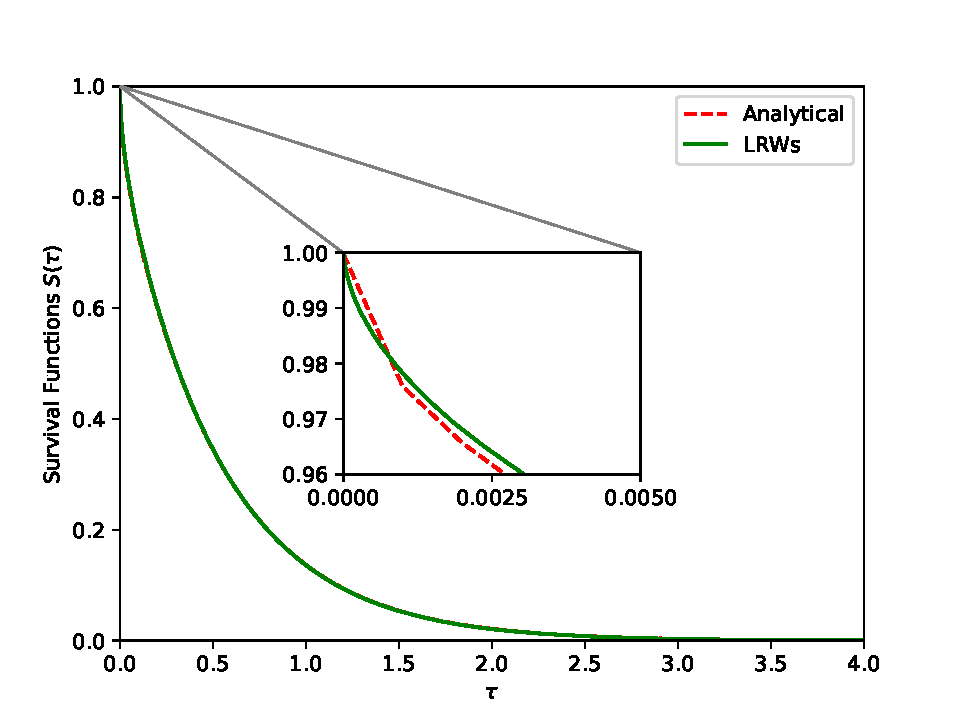
\includegraphics[width=0.8\textwidth]{LRWscheb}
    \caption{Survival curve for LRWs.\label{fig:LRW_survival}}
  \end{subfigure}
  \begin{subfigure}{0.9\textwidth}
    \centering
    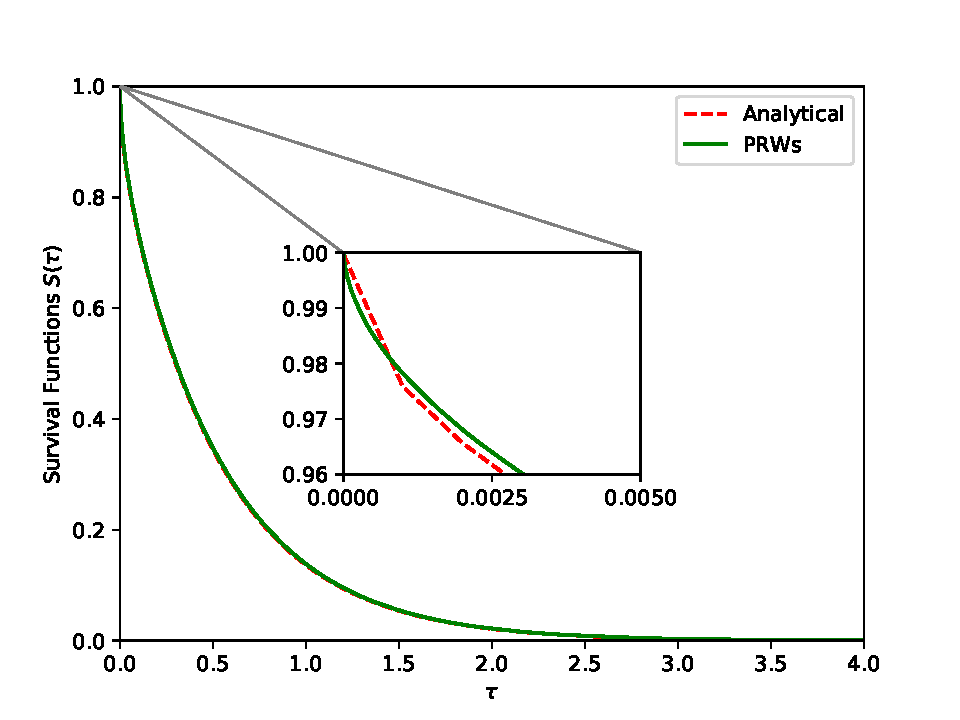
\includegraphics[width=0.8\textwidth]{PRWscheb}
    \caption{Survival curve for PRWs.\label{fig:PRW_survival}}
  \end{subfigure}
  \caption{Running PRWs and LRWs in the annulus with $1338643$
    particles determined by the Eq.~\ref{eq:cheb_sample_size} illustrating
    that the short and long time asypototic behaviors of the estimated
    survival functions of particles undergoing LRWs and PRWs are
    consistent with the analytical result in \highlight[{id=Yuge}]{Eq}}
  \label{fig:convergence_test}
\end{figure}

\begin{table}
  \centering
  \begin{tabular}{|c|c|c|}\hline
    Test Methods (standard nonparametric) & Statistics & P Values \\
    \hline
    Logrank & 0.017679 & 0.894223 \\
    \hline
    Fleming-Harrington & 0.742536 & 0.388850 \\
    \hline
    Gehan-Breslow & 0.742536 & 0.388850 \\
    \hline
    Tarone-Ware & 0.499418 & 0.479756 \\
    \hline
  \end{tabular}
  \caption{The estimated survival function of $1338643$ particles in
    the LRWs is statistically similar to the analytical survival
    function.}
  \label{tab:two_sample_test_lrws_analytical}
\end{table}

\begin{table}
  \centering
  \begin{tabular}{|c|c|c|}\hline
    Test Methods (standard nonparametric) & Statistics & P Values \\
    \hline
    Logrank & 0.039142 & 0.843168 \\
    \hline
    Fleming-Harrington & 0.083388 & 0.772757 \\
    \hline
    Gehan-Breslow & 0.083388 & 0.772757 \\
    \hline
    Tarone-Ware & 0.010582 & 0.918069 \\
    \hline
  \end{tabular}
  \caption{The estimated survival function of PRWs, which has
    $1338643$ particles with step length $0.5$, is not statistically
    different from the analytical survival function.}
  \label{tab:two_sample_test_prws_analytical}
\end{table}

From the visualized comparison in Figure~\ref{fig:convergence_test}
and the results of the two-sample statistical tests in
Table~\ref{tab:two_sample_test_lrws_analytical} and
Table~\ref{tab:two_sample_test_prws_analytical}, the fixed-step Monte
Carlo simulations' results converge to the analytical
outcomes. Therefore, the integral of the solutions of heat equations
can be approximated by the Monte Carlo simulations without calculating
manually. As mentioned in the last chapter, the integral, $S(\tau)$,
indicates the annulus' geometrical information. Therefore, the
fixed-time step Monte Carlo simulation can describe the shape of an
object without using the rulers. However, the number of particles in
the numerical simulations estimated by Eq.~\ref{eq:chab_substitute} is
abundant, which causes a high computational cost because each random
trajectories of each particle are simulated in LRWs and PRWs till they
reach the inner boundary of the annulus.


\subsubsection{Dvoretzky–Kiefer–Wolfowitz (DKW) inequality}

Chebyshev's inequality can be applied to any probability distribution,
but it is also weaker than other inequalities. DKW inequality is more
efficient since the confidence band is generated without running any
simulations. For example, let $F(\tau)$ be the true cumulative
distribution function (CDF) of the first passage time, a continuous unitless
random variable on the interval $[0, \infty]$. $F(\tau)$ has a
relationship with $S(\tau)$, which is

\begin{equation}\label{eq:cdf}
  F(\tau) = 1 - S(\tau)
\end{equation}

The true CDF is known by Eq.~\ref{eq:cdf}, which can also be approximated
numerically. A simple example of generating the CDF-based confidence
bounds by DKW inequality is shown in Figure~\ref{fig:dkw_cb_sample}. The empirical
distribution function $F_{256}(\tau)$ is estimated by the lifeline
module in Python \cite{davidson2019lifelines}. Thus, the interval
$\varepsilon$ contains the entire $F(\tau)$ with the probability
$95\%$ can be calculated by \highlight[id=Yuge]{Eq.$(2.20)$}

\begin{equation}\label{eq:dkw_cb}
  \varepsilon = \sqrt{\frac{\ln{\frac{2}{0.05}}}{2* 256}} \approx 0.084881
\end{equation}

\begin{figure}
  \centering
  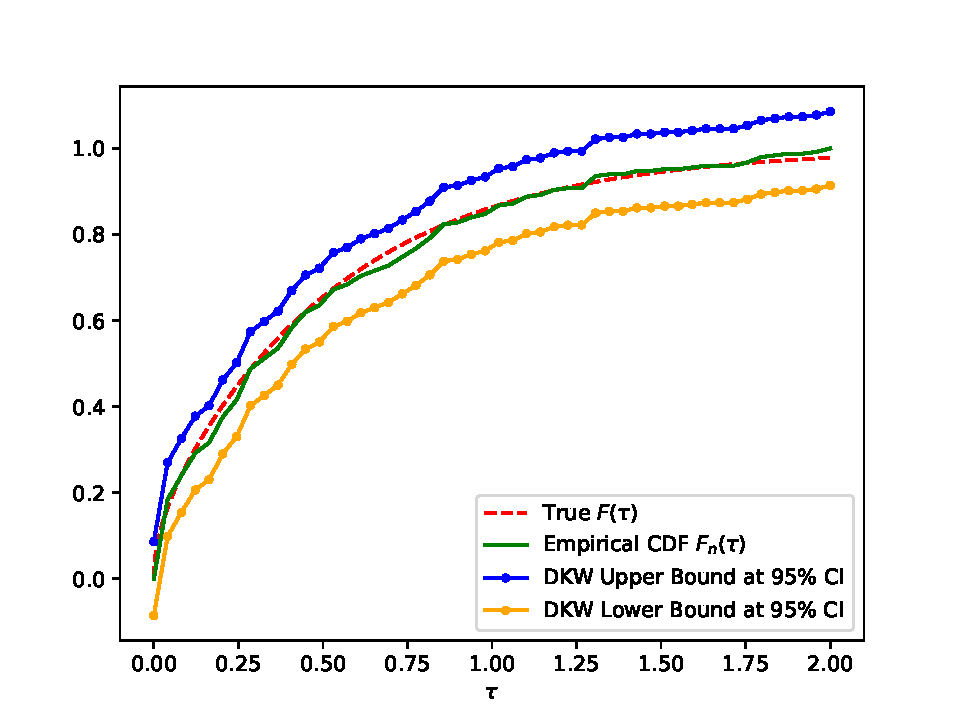
\includegraphics[width=0.8\textwidth]{dkw_comfidence_band_demo}
  \caption{The simultaneous band around $F_{256}(\tau)$ with interval
    $0.084881$ calculate by Eq.~\ref{eq:dkw_cb} encompasses
    the entire $F(x)$ at $95\%$ confidence level. \label{fig:dkw_cb_sample}}
\end{figure}



Moreover, the sample size estimated by DKW inequality \highlight[id=Yuge]{Eq.$(2.20)$} does
not depend on the geometries or the kind of simulations because the
simultaneous confidence bounds always contain the true cumulative
distribution at a specific confidence level. For instance, assume the
probability, that the maximum distance between $F_N(\tau)$ and
$F(\tau)$ is bigger than $0.005$, is smaller than $0.01$, the minimum
required number of particles should meet the inequality

\begin{equation}\label{eq:dkw_substitute}
  Pr(\sup_{x \in \mathbb{R}} |F_{N}(\tau) - F(\tau)| > 0.005) \leq 2e^{-2N0.005^2} = 0.01
\end{equation}

Thus, after the transformation of Eq.~\ref{eq:dkw_substitute}, the
sample size can be determined by

\begin{equation}\label{eq:dkw_sample_size}
  N \geq \frac{\ln(\frac{0.01}{2})}{-2 \times 0.005^2} \approx
  105966
\end{equation}


\begin{figure}
  \begin{subfigure}{0.9\textwidth}
    \centering
    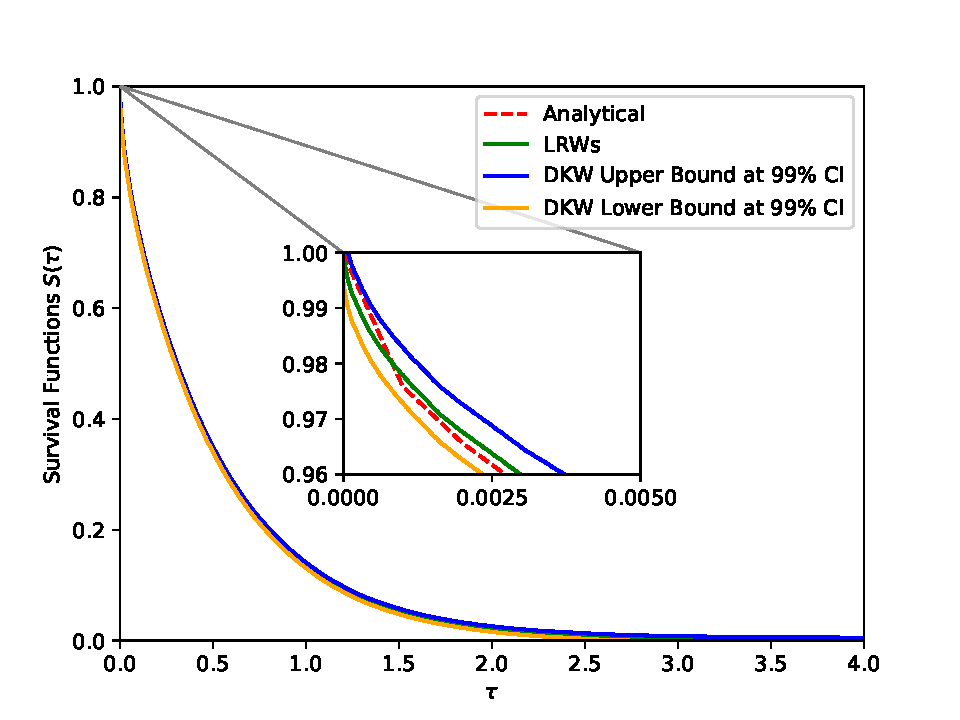
\includegraphics[width=0.8\textwidth]{LRWsdkw}
    \caption{The simultaneous confidence bands, generated by
      Eq.~\ref{eq:dkw_substitute}, of the estimated survival function
      $S(t)$ for LRWs contain the whole ture analytical
      $S(\tau)$. \label{fig:dkw_lrws_analytical}}
  \end{subfigure}
  \begin{subfigure}{0.9\textwidth}
    \centering
    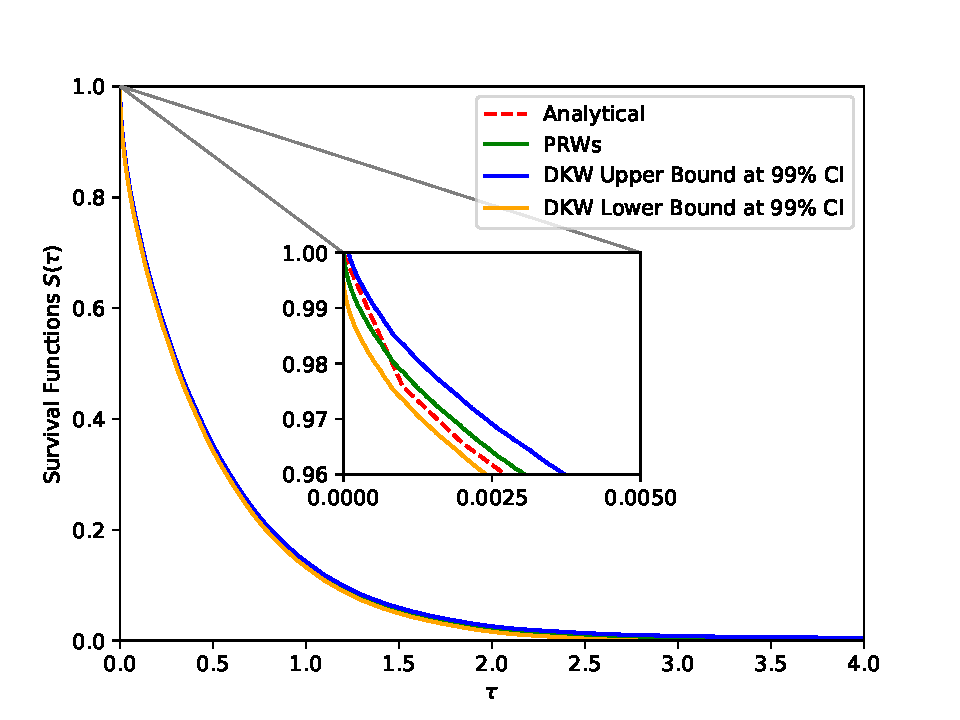
\includegraphics[width=0.8\textwidth]{PRWsdkw}
    \caption{The simultaneous confidence bands, generated by
      Eq.~\ref{eq:dkw_substitute}, of the estimated survival function
      $S(t)$ for PRWs contain the whole ture analytical
      $S(\tau)$. \label{fig:dkw_prws_analytical}}
  \end{subfigure}
  \caption{PRWs and LRWs are implemented in the annulus with $105966$
    particles determined by the Eq.~\ref{eq:dkw_sample_size}. (a) and
    (b) show that the DKW simultaneous confidence bands of estimated
    survival function with the interval $0.005$ encompass the entire
    analytical $S(\tau)$ at $99 \%$ confidence level. \label{fig:dkw_rw_analytical}}
\end{figure}

\begin{table}
  \centering
  \begin{tabular}{|c|c|c|}\hline
    Test Methods (standard nonparametric) & Statistics & P Values \\
    \hline
    Logrank & 1.532224 & 0.215779 \\
    \hline
    Fleming-Harrington & 1.630358 & 0.201654 \\
    \hline
    Gehan-Breslow & 1.630358 & 0.201654 \\
    \hline
    Tarone-Ware & 1.619530 & 0.203157 \\
    \hline
  \end{tabular}
  \caption{The estimated survival function of $105966$ particles in
    the LRWs is not statistically different to the analytical survival
    function.}
  \label{tab:two_sample_test_dkw_lrws_analytical}
\end{table}


\begin{table}
  \centering
  \begin{tabular}{|c|c|c|}\hline
    Test Methods (standard nonparametric) & Statistics & P Values \\
    \hline
    Logrank & 2.645624 & 0.103835 \\
    \hline
    Fleming-Harrington & 1.473674 & 0.224767 \\
    \hline
    Gehan-Breslow & 1.473674 & 0.224767 \\
    \hline
    Tarone-Ware & 1.986810 & 0.158675 \\
    \hline
  \end{tabular}
  \caption{The estimated survival function of PRWs, which has
    $105966$ particles with step length $0.5$, is statistically
    similar to the analytical survival function.}
  \label{tab:two_sample_test_dkw_prws_analytical}
\end{table}

From the Figure~\ref{fig:dkw_rw_analytical},
Table~\ref{tab:two_sample_test_dkw_lrws_analytical}, and
Table~\ref{tab:two_sample_test_dkw_prws_analytical}, although the sample
size in the LRWs and PRWs determined by DKW inequality is about $10$
times smaller than that by Chebyshev’s inequality, the estimated
survival functions of the numerical simulations converge to the
analytical results within the amount of statistical uncertainty.
 % subsection 2
  %
\subsection{Conclusion}


Instead of calculating the asymptotic expansion of the heat content
manually as $\tau \rightarrow 0^+$, the total heat energy $\beta$
\cite{gilkey1994heat} for time $\tau > 0$ can be approximated by the
fixed-time step Monte Carlo simulations for describing the full-scale
geometrical features of the annulus. Moreover, the required
number of particles in the simulations determined by the DKW
inequality is much smaller than the superabundant value estimated by
Chebyshev’s inequality.
 % subsection 3

  %__________ Section 3: Assumption Verification _______________________
  %\section{Assumption Verification}


....



\subsection{Circle and Rectangular}


...



\subsection{Branching Structures}


...


\subsection{Conculsion}



  
  
  %__________ Section 4: Conclusion _______________________
  %\section{Conclusion}

...








  % The Bibliograpy should go here. BEFORE appendices!
  %
  % I am not sure if alphabetical ordering is required, but it
  % certainly makes the text difficult to read, especially where
  % one has multiple references in a single \cite{} command.
  %
  %\bibliographystyle{unsrt}
  \uofsbibliography{thesisref}




  %%%%%%%%%%%%%%%%%%%%%%%%%%%%%%%%%%%%%%%%%%%%%%%%%%%%%%%%%%%%%%%%%%%%%%%%%
% APPENDICES
%
% Any chapters appearing after the \appendix command get numbered with
% capital letters starting with appendix 'A'.
% New chapters from here on will be called 'Appendix A', 'Appendix B'
% as opposed to 'Chapter 1', 'Chapter 2', etc.
%%%%%%%%%%%%%%%%%%%%%%%%%%%%%%%%%%%%%%%%%%%%%%%%%%%%%%%%%%%%%%%%%%%%%%%%%%

% Activate thesis appendix mode.
%\uofsappendix

% Put appendix chapters in the appendices environment so that they appear correcty
% in the table of contents.  You can use \input's here as well.

%\begin{appendices}

%\chapter{Sample Appendix}

%Stuff for this appendix goes here.

%\chapter{Another Sample Appendix}

%Stuff for this appendix goes here.

%\end{appendices}

\end{document}
